\documentclass[9pt,shortpaper,twoside,web]{ieeecolor2}
\usepackage{generic}
\usepackage{cite}
\usepackage{amsmath,amssymb,amsfonts}
\usepackage{graphicx}
\usepackage{textcomp}
\usepackage{booktabs}
\usepackage{multirow}
\usepackage{array}
\usepackage{algorithm}
\usepackage{algpseudocode}
\usepackage{xcolor}
\usepackage{url}

% --- editing macros: remove before submission -------------------------
\newcommand{\tbd}[1]{\textcolor{red}{[TODO: #1]}}
\newcommand{\NUMQ}[1]{\textcolor{red}{[NUMBER?: #1]}}
\newcommand{\NQ}{\textcolor{red}{[?]}}
% notation: frame {A}; transform of frame {B} with respect to {A}
\newcommand{\Tf}[2]{{}^{#1}\mathbf{T}_{#2}}
\newcommand{\Ch}{\hat{C}}% camera frame implied by the hand--eye calibration
\newcommand{\Tcorr}{\Tf{C}{\Ch}}% camera correction
% session names
% phantom dataset
\newcommand{\Pdata}{P}
\newcommand{\Pref}{P-ref}
\newcommand{\Prearra}{P-rearr1}
\newcommand{\Prearrb}{P-rearr2}
\newcommand{\Ppeople}{P-people}
\newcommand{\Pempty}{P-empty}
% forearm datasets
\newcommand{\Fone}{F1}
\newcommand{\Fval}{F1-val}
\newcommand{\Ftest}{F1-test}
\newcommand{\Ftwo}{F2}
\newcommand{\Fnew}{F2-new}
\newcommand{\Fsmall}{F2-small}
\newcommand{\Flarge}{F2-large}
\newcommand{\Fsubj}{F2-subj2}
\newcommand{\Farm}{F2-arm}
% ORB-SLAM3 modes
\newcommand{\fullslam}{\emph{full SLAM}}
\newcommand{\loconly}{\emph{localisation only}}
\newcommand{\reloc}{\emph{each frame relocalised}}

\def\BibTeX{{\rm B\kern-.05em{\sc i\kern-.025em b}\kern-.08em
    T\kern-.1667em\lower.7ex\hbox{E}\kern-.125emX}}
\markboth{\journalname, VOL. XX, NO. XX, XXXX 2026}
{Li \MakeLowercase{\textit{et al.}}: Probe-Mounted RGB-D Tracking by Self-Mapped Scene Coordinate Regression}

\begin{document}
\title{Freehand 3D Ultrasound Without an External Tracker: Probe-Mounted RGB-D Tracking by Self-Mapped Scene Coordinate Regression}

\author{Ruixuan~Li, Yipeng~Hu, and Emmanuel~Vander~Poorten%
\thanks{R. Li and E. Vander Poorten are with the Robot-Assisted Surgery group, KU Leuven, Leuven, Belgium (e-mail: ruixuan.li@kuleuven.be).}%
\thanks{Y. Hu is with the Dept of Med Phys \& Biomedical Eng, UCL, London, UK}
\thanks{This project received funding from FWO projects 12A8N26N and V444626N.}}

\maketitle

\begin{abstract}
\textcolor{cyan}{Objective:} Freehand three-dimensional (3D) ultrasound (US) requires the six-degree-of-freedom pose of every image, usually from an external tracker. This paper investigates whether a probe-mounted RGB-D camera alone can track the probe, and when it suffices for 3D compounding. \textcolor{cyan}{Methods:} The operator first scans the room with the probe camera (1--2\,min). One scene coordinate regression network learns the room from this scan without a tracker: it labels its own training data and localises each frame by a Kabsch RANSAC fit to the measured depth. Experiments used 63 test sweeps in one room, 32 on a phantom with controlled room changes and 31 on the forearms of two volunteers, against an optical tracker. \textcolor{cyan}{Results:} With a room scan covering the examination views in a furnished room, the error was 2.2--3.1\,mm (shape 1.7--1.9\,mm), 0.3--0.5\,mm above the same network trained on tracker poses; in an emptied room it was 5.85\,mm. A scan missing these views raised the error on the same sweeps from 2.28 to 13.57\,mm. With an occluder covering 30--60\,\% of the image width, the mean error rose by at most 0.9\,mm (no sweep above 8.5\,mm), whereas ORB-SLAM3, more accurate on most sweeps, lost single sweeps by 13--132\,mm while reporting tracking. \textcolor{cyan}{Conclusion:} Self-mapped per-frame localisation is a feasible tracker-free alternative when the room scan covers the examination views, with a bounded error and detectable failures. \textcolor{cyan}{Significance:} It removes external tracking hardware; its operating conditions give a scanning protocol with pre-examination checks.
\end{abstract}


\begin{IEEEkeywords}
Freehand 3D ultrasound, probe tracking, scene coordinate regression, RGB-D camera, visual relocalisation.
\end{IEEEkeywords}


\section{Introduction}
\label{sec:introduction}

\IEEEPARstart{U}{ltrasound} (US) imaging is widely used in diagnosis and intervention because it is real-time, free of ionising radiation, portable and inexpensive. However, a conventional probe shows a single 2D plane, and the operator has to build the 3D anatomy mentally from a sequence of images. Three-dimensional (3D) US provides organ and lesion volumes, vessel courses and planes for needle guidance \cite{Jiang2023}. Freehand 3D US obtains such volumes with a conventional probe: the operator sweeps the probe, and the 2D images are compounded into a 3D volume. This requires the six-degree-of-freedom (6-DoF) pose of every image \cite{solberg2007freehand}.

In practice, this pose comes from an optical or electromagnetic (EM) tracker \cite{solberg2007freehand}. An optical tracker needs a line of sight, which the operator or the staff may interrupt. An EM tracker needs a field generator near the patient, and metal nearby may disturb its field \cite{sorriento2019optical}. Both must be installed and calibrated in each room. This rules them out where a volume would be useful at short notice, such as at the bedside or in a crowded operating room \cite{blaivas2004bedside}. Thus, it is important to investigate probe tracking that gives an absolute pose for every frame without external hardware in the room.

Sensorless methods estimate the probe motion from the US images themselves: classically from speckle decorrelation \cite{gee2006sensorless}, and with deep networks from consecutive frames \cite{prevost2018}, multi-frame context \cite{guo2023tbme} or longer temporal context \cite{li2024longterm}. A coupling pad with N-shaped lines adds a reference visible in the image \cite{dai2024coupling}. Without such a reference, these methods integrate relative motion, so the error grows along the sweep. Trackers thus give an accurate pose at the cost of hardware in the room, and sensorless methods need no hardware at the cost of drift. Learned methods must also generalise across subjects and protocols. Thus, an absolute reference outside the US image is still needed.

A camera mounted on the probe sees the surroundings and can provide this reference. RGB-D cameras are small and inexpensive, and their depth gives metric 3D structure in every frame. Sun et al.\ \cite{sun2014skin} tracked skin features and built a skin map by visual SLAM; the poses are relative to the skin, and errors accumulate with the distance travelled. Visual--inertial odometry needs no prepared scene, but it drifts \cite{buchanan2024vio,he2024probemounted}. Absolute camera-based methods rely on something prepared in advance. ProbeSight localises a probe camera against a prior high-resolution surface map of the anatomy by inverse rendering \cite{wang2017probesight}. Huang et al.\ \cite{huang2025lightweight} regress the probe pose from two lightweight cameras relative to a workspace with coloured markers. Zhang et al.\ align camera images with a simulated replica of a textured workspace \cite{zhang2025servoing} and combine global visual guidance with local B-mode cues \cite{zhang2026seeing}. MLRecon tracks the probe from an external RGB-D camera without markers \cite{zhang2026mlrecon}, which brings back the line-of-sight constraint. Thus, existing camera-based methods either drift or depend on a prepared scene, a prior model of the anatomy or an external camera.

Busam et al.\ \cite{busam2018insideout} mounted an RGB-D camera of the same family on a transrectal probe, facing away from the patient. They tracked it by visual SLAM against a map of the operating room and compared the resulting 3D US compounding with an optical tracker. The room itself can therefore serve as the reference. Keypoint-based SLAM systems such as ORB-SLAM3 \cite{campos2021orbslam3} combine frame-to-frame tracking, keyframe selection, bundle adjustment, loop closing and place recognition, and carry a tracking state from frame to frame. When this state is wrong, for example after a hand has blocked part of the view, the error is carried into the following frames and may go undetected. For compounding, a silent failure of a whole sweep is harder to handle than a known, bounded error. Thus, it is important to investigate a room-referenced tracker that estimates the pose of every frame independently.


\begin{figure*}[t]
  \centering
  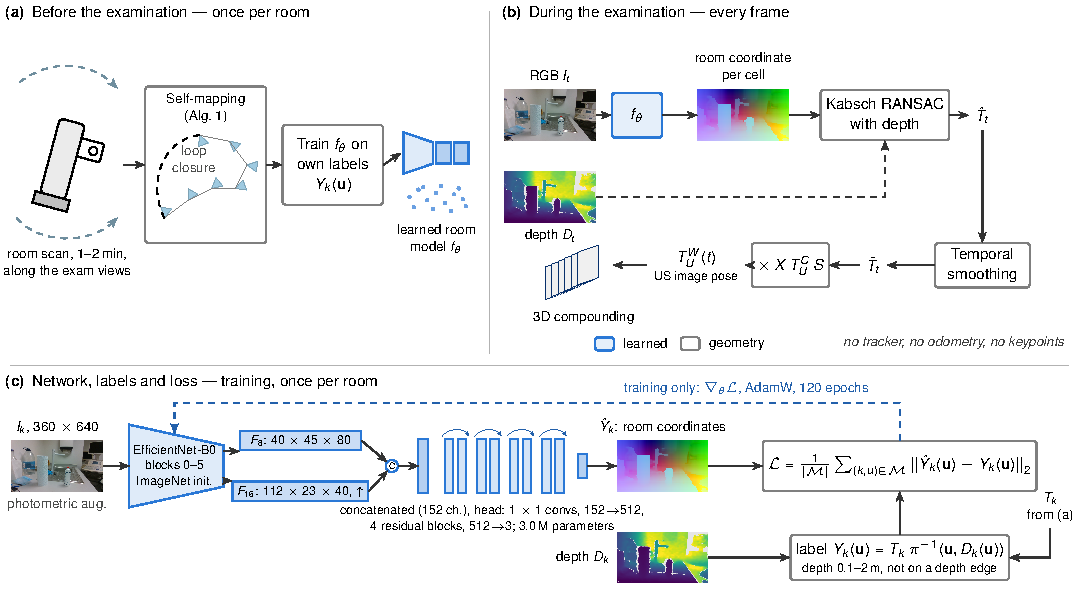
\includegraphics[width=\textwidth]{fig_overview.pdf}
  \caption{System overview. (a)~Before the examination: the room scan is self-mapped (Algorithm~\ref{alg:mapping}) and the network is trained on the resulting labels. (b)~During the examination: per-frame scene coordinates, Kabsch RANSAC with the measured depth, temporal smoothing and the probe calibration give the pose of the US image. (c)~Network, labels and loss (Eqs.~\eqref{eq:features}--\eqref{eq:loss}).}
  \label{fig:overview}
\end{figure*}

Learned visual relocalisation estimates an absolute pose from each scene image independently without a tracking state. Absolute pose regression (APR) maps an image directly to a pose \cite{7410693}. However, such networks behave more like image retrieval than geometric estimation, which limits their accuracy \cite{sattler2019}. Scene coordinate regression (SCR) instead predicts dense image-to-scene correspondences and solves the pose robustly. It was introduced with regression forests on RGB-D images \cite{shotton2013}, adapted to new scenes online \cite{cavallari2017onthefly,cavallari2019online}, trained end to end through a differentiable RANSAC in DSAC* \cite{brachmann2022dsac}, and improved for viewpoints far from the mapping images by ACE-G \cite{bruns2025aceg}. ACE0 removes the need for mapping poses by alternating between training the relocaliser on the images registered so far and registering further images with it \cite{brachmann2024ace0}. ACE-SLAM uses SCR as the map of a real-time RGB-D SLAM system \cite{alzugaray2025aceslam}. Relocalisation against a prior reconstruction has been studied in endoscopy, where the map is of the anatomy \cite{mahmoud2016orbslam}. 

To the best of the authors' knowledge, SCR has not yet been used to track the probe in freehand 3D US. Thus, this paper proposes a tracker-free approach for freehand 3D US reconstruction. A probe-mounted RGB-D camera scans the room before the examination and one SCR network learns the room from this scan. The approach is self-supervised because its labels come from the network's own pose estimates and the measured depth rather than from a tracker. The network learns the room, not the anatomy, so it needs no training data from other subjects. Every frame is localised on its own, so a wrong pose is not carried forward. The accuracy is set by the map before the first sweep. This paper therefore also studies how the room scan should be recorded, and when the approach is accurate enough for compounding. The contributions of this paper are listed as follows:
\begin{itemize}
  \item investigation of the feasibility of tracker-free freehand 3D US with a probe-mounted RGB-D camera and a room-referenced SCR network.
  \item development of a self-supervised mapping method, in which one SCR network learns a room from a short scan of it, labelled by its own poses and the measured depth.
  \item identification of the operating conditions of the approach (coverage of the examination views, map quality, scene changes and occlusion), and a resulting room-scan protocol with checks before the examination.
  \item experimental validation on phantom and forearm dataset of two volunteers against an optical tracker, separating the cost of mapping from that of tracking and the placement of the volume from its shape.
\end{itemize}
The rest of the paper is organised as follows. Section~\ref{sec:method} presents the proposed method. Section~\ref{sec:experiments} describes the experimental setup, the datasets, the experiment design and the evaluation criteria. Section~\ref{sec:results} reports the experimental results. Finally, the discussion and conclusion are given in Sections~\ref{sec:discussion} and~\ref{sec:conclusion}, respectively.




%======================================================================
\section{Method}
\label{sec:method}
%======================================================================
The proposed system has four components as shown in Fig.~\ref{fig:overview}. The scene coordinate network stores the room and predicts, for every image cell, the room point that the cell sees. The geometric solver computes the camera pose of a frame from these predictions and the measured depth. Self-mapping estimates the room-scan poses that label the network, without a tracker. Temporal smoothing and 3D compounding turn the per-frame poses into a volume. Self-mapping and training run once per room; the network, the solver and the smoothing then run on every sweep frame.


\subsection{Problem Statement and Notation}
\label{sec:notation}
The RGB-D camera is rigidly mounted on the US probe and faces the room as shown in Fig.~\ref{fig:overview}b. Before the examination, the operator records a \emph{room scan}, a set of $N$ RGB-D frames $\{(I_k,D_k)\}_{k=1}^{N}$, preferably along the planned sweep paths. During the examination, the operator records freehand sweeps, with frames $(I_t,D_t)$ indexed by $t$. Each camera frame consists of a colour image $I$ and a depth image $D$ aligned to it, and $\mathbf{K}$ denotes the colour intrinsics.

The accuracy of the approach rests on two assumptions. (i)~Most of the room surfaces seen by the camera are unchanged between the room scan and the sweeps. (ii)~The sweep views lie close to views of the room scan, because the network is trained only on those views. The camera mount is further assumed to stay rigid across sessions, and the room to contain enough depth structure for iterative closest point (ICP) registration.

The transformation $\Tf{A}{B}\in SE(3)$ denotes the frame $\{B\}$ with respect to the frame $\{A\}$. The pose of the US image frame $\{U\}$ in the map frame $\{W\}$, which is defined by the seed frame of self-mapping, is
\begin{equation}
  \Tf{W}{U}(t)=\Tf{W}{C}(t)\,\Tcorr\,\Tf{\Ch}{U} ,
  \label{eq:chain}
\end{equation}
\textcolor{red}{where $\Tf{W}{C}(t)$ is the estimated pose of the camera frame $\{C\}$. The camera correction $\Tcorr$ is a fixed transformation to $\{C\}$ from the camera frame $\{\Ch\}$ implied by the hand--eye calibration, and it makes the self-made map consistent with the probe calibration.} The camera-to-image calibration $\Tf{\Ch}{U}=(\Tf{M}{\Ch})^{-1}\,\Tf{M}{U}$ is composed of the hand--eye calibration $\Tf{M}{\Ch}$ and the US calibration $\Tf{M}{U}$, both relative to the marker frame $\{M\}$ on the probe. The matrix $\mathbf{S}=\mathrm{diag}(s,s,1,1)$ maps the homogeneous pixel coordinates of the US image to millimetres in $\{U\}$, with the pixel spacing $s$.  

The colour image is divided into a regular grid of square cells, with centres $\mathbf{u}$; a cell with depth $d$ is back-projected into $\{C\}$ by $\pi^{-1}(\mathbf{u},d)=d\,\mathbf{K}^{-1}[\mathbf{u}^\top,1]^\top$.  The poses $\mathbf{T}_k=\Tf{W}{C}(k)$ of the room-scan frames are unknown. The aim is to learn, from the room scan alone, a network $f_\theta$ and the poses $\{\mathbf{T}_k\}$, such that the camera pose of every sweep frame can be computed from that frame only,
\begin{equation}
  \big(\Tf{W}{C}(t),\,n_t\big)=g\big(f_\theta(I_t),\,D_t\big),
  \label{eq:problem}
\end{equation}
where $g$ is a fixed geometric solver and $n_t$ the inlier count of the pose. The pose of a frame therefore depends neither on earlier frames nor on a tracker.


\subsection{Scene Coordinate Network}
\label{sec:network}
A learned room model can give the pose in two other ways, by regressing the pose directly from the image, or by matching keypoints against a stored map. A pose-regression network compresses the whole image into one pose, so it cannot discard image regions that have changed, such as a hand in view \cite{sattler2019}. A keypoint map must be stored and matched for every frame. SCR keeps an exact geometric solver and learns only the correspondences, so that every cell gives its own 2D--3D correspondence and RANSAC can discard the cells that disagree. The network is then the map of the room; no point cloud or keyframe database is kept.

The network $f_\theta$, with $\theta=(\phi,\psi)$, consists of an encoder $E_\phi$ and a head $H_\psi$ (Fig.~\ref{fig:overview}c). The encoder is an ImageNet-pretrained EfficientNet-B0 \cite{tan2019efficientnet}, applied to the colour image resized to $360\times640$ and normalised with the ImageNet mean and standard deviation. It gives two feature maps $(\mathbf{F}_8,\mathbf{F}_{16})=E_\phi(I)$. The map $\mathbf{F}_8\in\mathbb{R}^{h_c\times w_c\times40}$ at stride 8 matches the cell grid of $h_c\times w_c=45\times80$ cells, each of $16\times16$ pixels of the full-resolution colour image. The map $\mathbf{F}_{16}$ at stride 16 has 112 channels and describes a larger image region around each cell. $\mathbf{F}_{16}$ is upsampled to the stride-8 grid by $\mathrm{Up}(\cdot)$, and the two are concatenated,
\begin{equation}
  \mathbf{F}=\big[\mathbf{F}_8,\ \mathrm{Up}(\mathbf{F}_{16})\big]\in\mathbb{R}^{h_c\times w_c\times152}.
  \label{eq:features}
\end{equation}
The head $H_\psi$ consists of $1\times1$ convolutions (152 to 512 channels, four residual blocks, 512 to 3 channels). A $1\times1$ convolution acts on each cell separately, so $H_\psi$ is one small multilayer perceptron applied to the feature vector of every cell; the context of a cell enters only through $\mathbf{F}$. The head predicts in metres relative to a fixed scene centre $\mathbf{c}$, the mean camera position of the training frames, so that its raw outputs are of order one for a room a few metres across. In millimetres, the predicted room points are, with $\mathbf{c}$ added to every cell,
\begin{equation}
  \hat{\mathbf{Y}}=f_\theta(I)=\mathbf{c}+10^{3}\,H_\psi(\mathbf{F})\in\mathbb{R}^{h_c\times w_c\times3},
  \label{eq:network}
\end{equation}
with $\hat{\mathbf{y}}(\mathbf{u})\in\mathbb{R}^3$ the entry of cell $\mathbf{u}$, i.e.\ the point of the room surface, in $\{W\}$, that this cell sees. One image thus gives up to $h_cw_c=3600$ correspondences for the solver $g$. The encoder is fine-tuned together with the head at a lower learning rate as summarized in Table~\ref{tab:params}. The head starts from PyTorch's default initialisation and runs in single precision; the encoder runs in mixed precision.

The underlying assumption is that the features of a cell identify the room surface it sees well enough for the head to map them to one room point. This holds for views similar to the training views, but not necessarily for new viewpoints, which is why assumption~(ii) matters. The network takes RGB only; depth enters the labels and the solver $g$, but not the network input.

\subsection{Training Labels and Loss}
\label{sec:training}
\subsubsection{Labels} Training needs, for every room-scan frame, the room point that each cell sees. Given the pose $\mathbf{T}_k$, this point follows from the measured depth by back-projecting the cell into $\{C\}$ and transforming it into $\{W\}$,
\begin{equation}
  \mathbf{y}_k(\mathbf{u})=\mathbf{T}_k\,\pi^{-1}\big(\mathbf{u},D_k(\mathbf{u})\big).
  \label{eq:label}
\end{equation}
The poses $\mathbf{T}_k$ come from self-mapping; with tracker poses instead, the same procedure gives the \emph{oracle map} used in the experiments. An error of $\mathbf{T}_k$ moves all labels of frame $k$ together, so the network can be no more accurate than the room-scan poses it is trained on.

A cell is labelled only if $0.1\,\mathrm{m}<D_k(\mathbf{u})<2$\,m and no neighbouring cell is more than 6\,\% nearer or farther, because at a depth edge the depth of a cell mixes two surfaces and would give a point in free space. Cells without a valid label are left out of the loss. The network still predicts a point for them, but at test time only cells with depth are used.

\subsubsection{Loss} The loss is the mean Euclidean distance over the labelled cells $\mathcal{M}$ of a batch,
\begin{equation}
  \mathcal{L}(\theta)=\frac{1}{|\mathcal{M}|}\sum_{(k,\mathbf{u})\in\mathcal{M}}\left\|\hat{\mathbf{y}}_k(\mathbf{u})-\mathbf{y}_k(\mathbf{u})\right\|_2 ,
  \label{eq:loss}
\end{equation}
with $\hat{\mathbf{y}}_k(\mathbf{u})$ the prediction of Eq.~\eqref{eq:network} for image $I_k$. The distance is not squared, so that its gradient keeps the same magnitude as the error approaches the millimetre scale and wrong labels that remain have less influence than with a squared error.

\subsubsection{Training} One network is trained per room on all its room-scan frames, so a new room requires a new room scan. Training uses AdamW with a linear warm-up, a constant learning rate and a cosine decay to zero, and the augmentation is photometric only (Table~\ref{tab:params}). One epoch passes once over all room-scan frames in random order. Self-mapping uses the same loss and settings with a fixed number of steps per round, and one network is trained on through all rounds. The final network is trained from scratch, starting from the ImageNet encoder, on the labels of the optimised poses.

\subsection{Per-Frame Pose Estimation}
\label{sec:pose}
Every cell $i$ with depth $d_i<2$\,m gives a camera point $\mathbf{x}_i=\pi^{-1}(\mathbf{u}_i,d_i)$ and a predicted room point $\hat{\mathbf{y}}_i=f_\theta(I)(\mathbf{u}_i)$; the correspondences are fixed by the cell grid, without keypoints or descriptors. For a set $\mathcal{S}$, the Kabsch fit \cite{kabsch1976}
\begin{equation}
  (\mathbf{R},\mathbf{t})=\arg\min_{\mathbf{R}\in SO(3),\,\mathbf{t}}\ \sum_{i\in\mathcal{S}}\|\mathbf{R}\mathbf{x}_i+\mathbf{t}-\hat{\mathbf{y}}_i\|^2
  \label{eq:kabsch}
\end{equation}
has a closed-form solution by singular value decomposition. The inliers of a pose are $\mathcal{I}=\{i:\|\mathbf{R}\mathbf{x}_i+\mathbf{t}-\hat{\mathbf{y}}_i\|<20\,\mathrm{mm}\}$. RANSAC \cite{fischler1981ransac} draws 256 samples of three correspondences and keeps the hypothesis with the most inliers. This hypothesis is refitted three times on its inliers, and the inlier set is re-evaluated after each refit. The final refit gives the pose $\hat{\mathbf{T}}_t$, composed of $(\mathbf{R},\mathbf{t})$, and the inlier count $n_t=|\mathcal{I}|$ (at most $h_cw_c$, the number of cells). The three cells of a sample are drawn uniformly at random from the cells with depth. Frames with $n_t<400$ receive no pose (the \emph{inlier gate}). No earlier pose is used as a prior, so errors cannot accumulate over a sweep. Together, these steps form the solver $g$ of Eq.~\eqref{eq:problem}.

\begin{algorithm}[t]
  \caption{Self-mapping of a room scan}
  \label{alg:mapping}
  \small
  \begin{algorithmic}[1]
    \Require RGB-D room scan $\{(I_k,D_k)\}_{k=1}^{N}$
    \Ensure room-scan poses $\{\mathbf{T}_k\}$ in the map frame $\{W\}$; network $f_\theta$
    \Statex \textit{Seed: define $\{W\}$ by depth alone}
    \State $k_0\gets$ first frame of the first video
    \Repeat
      \State $\mathbf{T}_{k_0}\gets\mathbf{I}_4$; chain depth ICP outwards over $\pm2$\,s
      \State $\mathcal{K}\gets$ frames placed by ICP
      \If{$\mathcal{K}$ spans less than 1\,s} $k_0\gets k_0+1$\,s \EndIf
    \Until{$\mathcal{K}$ spans 1\,s, or 20 tries (keep the best)}
    \Statex \textit{Rounds: grow the map with the network}
    \State $m\gets2000$
    \Repeat
      \State train $f_\theta$ on the labels of $\mathcal{K}$ for $m$ steps (Eq.~\eqref{eq:loss}); $m\gets1500$
      \ForAll{$k\notin\mathcal{K}$}
        \State $(\hat{\mathbf{T}}_k,n_k)\gets$ Kabsch RANSAC on $f_\theta(I_k)$ and $D_k$ (Sec.~\ref{sec:pose})
      \EndFor
      \State add $k$ within 150 frames of $\mathcal{K}$ if $n_k\ge60$ and its motion is plausible
      \State add every 30th remaining $k$ if $n_k\ge400$ \Comment{admits new videos}
      \State extend each segment of $\mathcal{K}$ by depth ICP, up to 90 frames per end
    \Until{fewer than 0.5\,\% of the frames were added}
    \Statex \textit{Refinement: remove the bending of the map}
    \State $\mathbf{T}^0_k\gets\hat{\mathbf{T}}_k$ for every frame with $n_k\ge400$
    \State $\mathcal{E}\gets$ sequential and loop-closure edges, each with an ICP pose $\mathbf{Z}_{ij}$
    \State remove edges whose $\mathbf{Z}_{ij}$ deviates from the map by more than 50\,mm
    \State $\{\mathbf{T}_k\}\gets$ minimiser of Eq.~\eqref{eq:posegraph} over $\mathcal{E}$
    \State train $f_\theta$ from scratch on the labels of $\{\mathbf{T}_k\}$
    \State \Return $\{\mathbf{T}_k\}$, $f_\theta$
  \end{algorithmic}
\end{algorithm}

\subsection{Self-Mapping Without a Tracker}
\label{sec:mapping}
% Self-mapping estimates all $\mathbf{T}_k$ from the RGB-D room scan alone (Algorithm~\ref{alg:mapping}), with the loss of Sec.~\ref{sec:training} and the pose estimation of Sec.~\ref{sec:pose}; several videos are mapped jointly into one frame.

The network cannot localise before it is trained, so the first frames are placed by depth alone. The seed frame defines $\{W\}$; the first try is the first frame of the first video. Frames within $\pm2$\,s of it are placed by chaining frame-to-frame point-to-plane ICP on the depth outwards from the seed \cite{chen1992icp,low2004linear}. ICP uses points on a 4-pixel grid with an inlier distance of 10\,mm, and an alignment is accepted if at least 50\,\% of the points are inliers with an RMS of at most 6\,mm. ICP is a custom implementation with linearised point-to-plane steps, nearest neighbours by a $k$-d tree and at most 8000 source points; it starts from the identity, since the frames are consecutive (iterations and distances in Table~\ref{tab:params}). If ICP places less than 1\,s of the scan, e.g.\ because a hand covers the camera, the seed moves 1\,s later, up to 20 times; if no try succeeds, the best one is used.

Each round trains the network on the set $\mathcal{K}$ of placed frames (2000 steps in the first round, 1500 afterwards) and localises the others with it. Two rules decide which frames join the map. Near the map, a low inlier threshold lets the map grow into views the network has seen only partly, and a motion check rejects the wrong poses this admits. A frame within 150 frames of a placed frame of the same video joins if it has $\ge60$ inliers and its implied motion is plausible, i.e.\ its pose differs from that of the nearest placed frame of the same video, $\Delta\tau$ apart, by at most $500\,\mathrm{mm/s}\cdot\Delta\tau+20$\,mm in position and $90^\circ/\mathrm{s}\cdot\Delta\tau+5^\circ$ in orientation. Far from the map, no motion check is possible, so every 30th remaining frame joins only if it passes the stricter inlier gate of Sec.~\ref{sec:pose} with at least 400 inliers. This rule admits a second video that has no ICP link to the first. Depth ICP then extends each placed segment by up to 90 frames at both ends, which places frames that the network does not yet localise. Mapping stops when a round adds fewer than 0.5\,\% of the frames. A final pass relocalises every frame with the same inlier gate as at test time and keeps the poses with at least 400 inliers as initial poses $\mathbf{T}^0_k$.



Independently localised frames are individually plausible, but the map bends over seconds. The graph combines the network poses with ICP relative poses $\mathbf{Z}_{ij}$ (the pose of frame $j$ with respect to frame $i$) over an edge set $\mathcal{E}$. \emph{Sequential} edges connect frames 1, 5, 15 and 30 apart, and \emph{loop-closure} edges connect frames that observe the same part of the room but lie more than 2\,s apart or in different videos. Each third frame gets up to three such partners whose camera centres and points 1\,m ahead both lie within 150\,mm. Each $\mathbf{Z}_{ij}$ is estimated by the point-to-plane ICP above, initialised with the relative pose of the two network poses. Edges whose $\mathbf{Z}_{ij}$ deviates from the map by more than 50\,mm are dropped, which removes failed ICP alignments before the optimisation. Each pose is written as 
\begin{equation}
\mathbf{T}_k=\mathbf{T}^0_k\begin{bmatrix}\mathrm{Exp}(\boldsymbol{\omega}_k)&\mathbf{v}_k\\\mathbf{0}^\top&1\end{bmatrix},
  \label{eq:param}
\end{equation}
where $\boldsymbol{\delta}_k=(\boldsymbol{\omega}_k,\mathbf{v}_k)\in\mathbb{R}^6$ and $\mathrm{Exp}(\cdot)$ maps a rotation vector to $SO(3)$. With the set $\mathcal{Q}$ of four points 1\,m in front of the camera and $\mathcal{P}=\mathcal{Q}\cup\{\mathbf{0}\}$, the graph solves
\begin{equation}
  \begin{aligned}
  \{\boldsymbol{\delta}_k^\ast\}=\arg\min_{\{\boldsymbol{\delta}_k\}}\ &\sum_{(i,j)\in\mathcal{E}}\sum_{\mathbf{p}\in\mathcal{P}}\bar{\rho}\big(\mathbf{e}_{ij}(\mathbf{p})/\sigma_e\big)\\
  +&\sum_{k}\sum_{\mathbf{q}\in\mathcal{Q}}\bar{\rho}\big(\mathbf{e}_{k}(\mathbf{q})/\sigma_p\big),
  \end{aligned}
  \label{eq:posegraph}
\end{equation}
where $\mathbf{e}_{ij}(\mathbf{p})=\mathbf{Z}_{ij}^{-1}\mathbf{T}_i^{-1}\mathbf{T}_j\mathbf{p}-\mathbf{p}$ is the edge residual and $\mathbf{e}_k(\mathbf{q})=\mathbf{T}_k\mathbf{q}-\mathbf{T}^0_k\mathbf{q}$ the prior residual, with $\sigma_e=1$\,mm and $\sigma_p=10$\,mm. The robust loss $\bar{\rho}(\mathbf{e})=\sum_{a\in\{x,y,z\}}\rho(e_a^2)$ with $\rho(z)=2(\sqrt{1+z}-1)$ acts on each coordinate of a residual. Eq.~\eqref{eq:posegraph} is solved by trust-region least squares with a sparse Jacobian (SciPy) for at most 300 function evaluations. Point residuals put all constraints in millimetres without a rotation weight, and the points ahead constrain orientation through what the camera sees. The prior fixes the gauge and keeps ICP failures from bending the map. The poses $\mathbf{T}_k$ that follow from $\{\boldsymbol{\delta}^\ast_k\}$ label the final network, which is trained from scratch so that it learns only from these labels (Sec.~\ref{sec:training}).


\subsection{Temporal Smoothing and 3D Compounding}
\label{sec:smoothing}
For frame $t$ at time $\tau_t$, every pose $j$ in a window with $\Delta_j=\tau_j-\tau_t$ receives the weight
\begin{equation}
  w_j=n_j\big(1-|\Delta_j/\Delta_h|^3\big)^3\big[1-(r_j/\kappa)^2\big]_+^2 ,
  \label{eq:weights}
\end{equation}
where $n_j$ is the inlier count and $\Delta_h$ is the half-width of the window offline and its full length in real time, widened to the farthest pose if fewer than three poses fall in the window. The last factor is a Tukey weight with $[x]_+=\max(x,0)$, which is 1 in the first fit and is updated in two reweightings to make the fit robust. The residual $r_j$ adds the translation residual in mm and 0.16\,mm per mrad of rotation residual (the lever arm to the image), and $\kappa$ is six times the median residual. The translations $\mathbf{t}_j$ are fitted by a weighted polynomial of degree $\ell$ in $\Delta_j$,
\begin{equation}
  \{\mathbf{b}_l\}=\arg\min_{\{\mathbf{b}_l\}}\sum_j w_j\Big\|\mathbf{t}_j-\sum_{l=0}^{\ell}\mathbf{b}_l\,\Delta_j^{\,l}\Big\|^2 ,
  \label{eq:smoothing}
\end{equation}
with $\ell=2$ if at least five poses surround $\tau_t$, $\ell=1$ with three or four, and $\ell=0$ otherwise. The smoothed translation is $\mathbf{b}_0$, the value of the fit at $\tau_t$. Rotations are fitted in the same way, as rotation vectors about the weighted mean rotation. Together they give the smoothed pose $\bar{\mathbf{T}}_t$. Offline, the window is centred, $|\Delta_j|\le1$\,s. In real time, the pose of frame $t$ is output 0.25\,s later from the last 1\,s of poses, $\Delta_j\in[-0.75,0.25]$\,s. This fit uses Eq.~\eqref{eq:smoothing} with $\ell=1$ for at least five poses and $\ell=0$ otherwise, evaluated at $\tau_t$. The fully causal variant uses the last 0.25\,s, $\Delta_j\in[-0.25,0]$\,s.

Each US pixel is placed in $\{W\}$ by $\Tf{W}{U}(t)\,\mathbf{S}$, with Eq.~\eqref{eq:chain} evaluated at the smoothed pose $\bar{\mathbf{T}}_t$, and added to the nearest voxel of a 0.4\,mm grid. The grid is aligned with the sweep, with its axes along the mean lateral, axial and elevational directions of the reference images and its origin at their centre. Pixels in the same voxel are averaged, and empty voxels are left empty. Reference volumes are compounded in the same way from the tracker poses. For display, a 6\,mm slab centred on the sweep is shown as a maximum-intensity projection along the viewing direction.

\begin{table}[t]
  \caption{Main parameters of the proposed system.}
  \label{tab:params}
  \centering
  \begin{tabular}{@{}llr@{}}
    \toprule
    Stage & Parameter & Value\\
    \midrule
    Training & optimiser, batch size & AdamW, 8\\
     & learning rate, head / encoder & $10^{-3}$ / $10^{-4}$\\
     & weight decay & $10^{-4}$\\
     & epochs & 120\\
     & warm-up / constant rate until & 1 / 60\,\% of steps\\
     % & augmentation: brightness, contrast, gain & $\pm0.2$, 0.8--1.2, 0.9--1.1\\
     & valid label depth & 0.1--2\,m\\
    \midrule
    Pose & RANSAC samples & 256\\
     & inlier distance & 20\,mm\\
     & inlier gate & 400\\
    \midrule
    Self-mapping & seed window & $\pm2$\,s\\
     & steps, first / later rounds & 2000 / 1500\\
     & inliers to join, near / far & 60 / 400\\
     & stop when new frames below & 0.5\,\%\\
     & ICP iterations, distance & 10, 40$\to$10\,mm\\
    \midrule
    Pose graph & sequential edges (frames apart) & 1, 5, 15, 30\\
     & loop-closure radius & 150\,mm\\
     & edge rejection & 50\,mm\\
     & $\sigma_e$ / $\sigma_p$ & 1 / 10\,mm\\
    \midrule
    Smoothing & window, offline & $\pm1$\,s\\
     & window, real time & $-0.75$ to $+0.25$\,s\\
    \midrule
    Compounding & voxel size & 0.4\,mm\\
    \bottomrule
  \end{tabular}
\end{table}




%======================================================================
\section{Experiments and Evaluation}
\label{sec:experiments}
%======================================================================

\subsection{Experimental Setup}
\label{sec:implementation}
US data were acquired on an Ultrasonix machine (BK, Europe) with a curvilinear probe (4DC7-3/40). B-mode images of $640\times480$ pixels were grabbed from the scanner at 20 frames/s, with a depth of 9\,cm and a pixel spacing of 0.23\,mm; the frequency was 6\,MHz with median speckle reduction and persistence 3. A RealSense D435i RGB-D camera (Intel Corp., Santa Clara, CA, USA) was rigidly mounted on the probe by a 3D-printed holder; it recorded colour images of $1280\times720$ pixels at about 30\,Hz, with depth aligned to colour by the RealSense SDK. An optical tracker (Polaris Vega, Northern Digital Inc., Waterloo, ON, Canada) tracked a passive marker on the probe; it provides the calibration and the ground truth (GT) and is not used by the proposed system during the examination.

The method is implemented in PyTorch and runs on one RTX A4500 GPU (NVIDIA Corp., Santa Clara, CA, USA). Self-mapping takes about 30\,min per room and training the final network about 40\,min for 120 epochs. Table~\ref{tab:params} lists the main parameters of the proposed system.

\subsection{Calibration, Synchronisation and Ground Truth}
\label{sec:calib}\label{sec:groundtruth}\label{sec:sensorcal}
The probe marker serves the one-off calibration and the GT. The hand--eye calibration $\Tf{M}{\Ch}$ was estimated by fitting it jointly with the board pose, by robust least squares, to the corners of a fixed ChArUco board ($12\times9$ squares of 15\,mm) in the still frames of two calibration sessions (3.5\,mm error at the board corners), and the US calibration $\Tf{M}{U}$ by a pinhead-based method \cite{TODO-us-calibration}. Tracker, camera and US images were synchronised by ROS message filter and matched by nearest timestamp; no residual offset remained (best shift $+3$ to $+9$\,ms).

In the tracker frame $\{O\}$, which serves only the calibration and the evaluation, the tracker measures the camera through the hand--eye calibration, $\Tf{O}{\Ch}(k)=\Tf{O}{M}(k)\,\Tf{M}{\Ch}$. For a tracker-made map, an error of $\Tf{M}{\Ch}$ cancels, as labels, GT and $\Tf{\Ch}{U}$ share the same displaced frame $\{\Ch\}$; a self-made map refers to the physical camera $\{C\}$, so the error remains as the camera correction $\Tcorr$. It is estimated jointly with the alignment $\mathbf{A}=\Tf{O}{W}$ of $\{W\}$ to $\{O\}$ over the room-scan frames,
\begin{equation}
  (\mathbf{A},\Tcorr)=\arg\min_{\mathbf{A},\,\Tcorr\in SE(3)}\sum_k\sum_{\mathbf{p}\in\mathcal{P}}\bar{\rho}\Big(\big(\mathbf{A}\,\mathbf{T}_k\,\Tcorr\,\mathbf{p}-\Tf{O}{\Ch}(k)\,\mathbf{p}\big)/\sigma_c\Big),
  \label{eq:calib}
\end{equation}
with $\bar{\rho}$ and $\mathcal{P}$ as in Eq.~\eqref{eq:posegraph} and $\sigma_c=5$\,mm, initialised by ten alternating steps ($\mathbf{A}$ by a Kabsch fit, $\Tcorr$ from the mean rotation and median translation of the per-frame offsets). $\Tcorr$ is fitted once on \Ftest{} and reused unchanged on all other sets. $\mathbf{A}$ is used for evaluation only.
 

\begin{table}[!tb]
  \caption{Datasets, all recorded in one room. Cov.: share of sweep viewpoints covered by the room scan (Sec.~\ref{sec:protocol}).}
  \label{tab:data}
  \centering
  \footnotesize
  \setlength{\tabcolsep}{3pt}
  \begin{tabular}{@{}lcl cc l@{}}
    \toprule
    & & & \multicolumn{2}{c}{Cov.\ (\%)} & \\
    \cmidrule(lr){4-5}
    Set & Sweeps & Map from & Exam & Gen. & Room at sweep time \\
    \midrule
    \multicolumn{6}{@{}l}{\emph{Forearm, exam-view room scans, 2.0--3.0\,min}}\\
    \Fval{}  & 2 & own & -- & -- & same day, settings only \\
    \Ftest{} & 5 & own & 93--96 & -- & few objects moved \\
    \midrule
    \multicolumn{6}{@{}l}{\emph{Phantom: exam-view and generic room scan per set}}\\
    \Pref{}    & 8 & own & 96 & 0  & unchanged \\
    \Prearra{} & 8 & own & 75 & 93 & large rearrangement \\
    \Prearrb{} & 8 & own & 96 & 78 & very large rearrangement \\
    \Ppeople{} & 4 & \Prearrb{} & 98 & 100 & people moving \\
    \Pempty{}  & 4 & own & 92 & 97 & room emptied \\
    \midrule
    \multicolumn{6}{@{}l}{\emph{Forearm, generic room scans, 40--90\,s}}\\
    \Fnew{}   & 8 & own & -- & $\le$14 & new session \\
    \Fsmall{} & 4 & own & -- & $\le$14 & small room change \\
    \Flarge{} & 4 & own & -- & $\le$14 & large room change \\
    \Fsubj{}  & 6 & \Flarge{} & -- & $\le$14 & second volunteer \\
    \Farm{}   & 4 & \Flarge{} & -- & $\le$14 & obstacle in view \\
    \bottomrule
  \end{tabular}
\end{table}

\subsection{Datasets and Protocol}
\label{sec:data}\label{sec:sessions}\label{sec:rules}\label{sec:protocol}
All data were recorded in one room, on a femur silicone phantom and forearms of volunteers.   \tbd{sweep direction, length and plane orientation, e.g.\ distal-to-proximal, 100--200\,mm, plane perpendicular to the forearm}. Table~\ref{tab:data} summarises the datasets. The phantom dataset changes one room condition at a time; the forearm datasets test the system in vivo. In total, 65 sweeps are evaluated: 2 for validation and 63 for testing (32 phantom and 31 forearm sweeps).
% This study was performed in accordance with the ethical standards of the 1964 Declaration of Helsinki and its later amendments. Approval was granted by \tbd{ethics committee} on \tbd{date} [\tbd{approval number}], and the volunteers gave informed consent.

The 32 sweeps form five sets, one per room condition: the reference \Pref{}; a large and a very large rearrangement of the furniture, \Prearra{} and \Prearrb{}; people moving in the background, \Ppeople{}, in the layout of \Prearrb{} and with its room scans; and the emptied room, \Pempty{}. Each set has two room scans. The \emph{exam-view} scan follows the protocol below: the probe is held in the air along each of the four sweep paths (views) at sweep height and angle. The \emph{generic} scan walks the room and tests the effect of coverage.

\Fval{} (2 sweeps) is used only to choose the settings. \Ftest{} (5 sweeps), later the same day with a few objects moved, is the in-vivo test with covering room scans. The 26 sweeps were recorded five days after \Fone{}, in five sets: a new session \Fnew{}, a small and a large room change, \Fsmall{} and \Flarge{}, the second volunteer \Fsubj{}, and an arm in view of the camera, \Farm{}. The room scans are short and generic, and \Fsubj{} and \Farm{} use the scans of \Flarge{}. \Ftwo{} is the uncontrolled case.


The procedure has three steps, motivated by the experiments (Sec.~\ref{sec:res_coverage}). (a)~\emph{Exam-view scan:} the operator records the room scan with the probe held in the air along each planned sweep path, at sweep height and angle. (b)~\emph{Coverage check:} after the first sweep, the share of sweep frames with a room-scan pose within 30\,mm (camera centre) and $10^\circ$ (orientation) is computed, searching all room-scan poses for each sweep frame; the examination proceeds if it is at least 80\,\%. (c)~\emph{Map-age check:} the median Kabsch inlier count $n_t$ over the frames of a set flags an outdated map, in which case the room is rescanned; in this study the median was computed over all sweep frames of the set.

All settings were chosen on \Fval{}, and the smoothing windows as the lowest error for their delay. Each network is trained on the room scan of its set only. Mapping and training use every frame of the room scan that has a tracker pose, so that every map pose can be evaluated against the tracker and the self-made and oracle maps are trained on the same frames. \Ftwo{} networks were also trained on all room scans of the day up to the set (\emph{pooled}; supplementary material). Seed spread was measured with three training seeds on \Ftest{} and on every phantom set. For the comparison with ORB-SLAM3, the systems are paired by sweep, and the mean difference is reported with a 95\,\% bootstrap interval and a Wilcoxon signed-rank test.

\subsection{Experiment Design}
Six experiments are reported. The first two test the system when both assumptions of Sec.~\ref{sec:notation} hold. The third relaxes assumption~(ii), and the fourth and fifth relax assumption~(i). The sixth compares the system with other trackers.

\emph{1) Accuracy with covering room scans.} Every phantom set is tracked with its exam-view scan, and \Ftest{} with its own room scans. The results are compared with the \emph{oracle map}, the same network trained on tracker poses of the room scan, which isolates mapping from tracking. On \Ftest{}, the system is also evaluated using only the room scan recorded before the sweeps (\emph{strict protocol}) and with the real-time and causal smoothing.  

\emph{2) Ablations.} Self-mapping is repeated from scratch on \Ftest{} without loop closures and without the camera correction $\Tcorr$. The tracking settings are varied on \Fval{} with the oracle map: training length, PnP instead of Kabsch, geometric augmentation, input resolution and smoothing. $\Tcorr$ is fitted on each \Ftest{} scan alone, and refitted on \Flarge{}.

\emph{3) Coverage of the examination views.} On the phantom, the same sweeps are tracked with the exam-view scan, the generic scan and both scans in one map. Per frame, the anchor error is related to the distance to the nearest room-scan pose. On \Ftest{}, only the first 20, 40 and 60\,s of the room scans are mapped. \Ftwo{}, with short generic scans and a second volunteer, is the uncontrolled case.

\emph{4) Scene changes.} On the phantom, the map of an earlier set tracks the sweeps of a later set (\emph{outdated} map). \Ppeople{} adds people moving in the background, and on \Pref{} the room scan is also recorded after the sweeps.

\emph{5) Occlusion.} A synthetic occluder is added to the sweep frames of \Prearra{} and \Prearrb{} (16 sweeps), as by the operator's hand or arm. It is a band over the full image height and 30\,\% or 60\,\% of the image width, filled with a skin-like colour and a fixed texture, so that keypoint detectors find corners on it, at a depth of 0.4\,m. It appears for 3\,s every 10\,s, starting 5\,s into each sweep and alternating between the left and right side, so that about 30\,\% of the sweep time is occluded. The room scans are not occluded, and all systems receive identical frames. \Farm{}, with a real arm in view of the camera, is the real case.

\emph{6) Comparison with other trackers}, on all sets (Table~\ref{tab:baselines}). The first four systems use a map labelled with tracker poses, so that only the localisation differs. \emph{Classical pipeline:} SIFT \cite{lowe2004sift} matches against room-scan keyframes, lifted to 3D with depth and solved by PnP-RANSAC \cite{lepetit2009epnp}, with SIFT RGB-D odometry in between and a pose graph \cite{liu2025rgb}. \emph{Pose regression:} a network that regresses the pose between a keyframe and the query, with learned odometry \cite{TODO-own-pose-regression}. \emph{Hybrid:} the per-frame SCR poses as anchors in the SIFT odometry with a pose graph. \emph{Odometry only:} SIFT odometry with each segment start posed by the tracker, a lower bound without a map. The remaining systems need no tracker. The classical pipeline is also run on the self-made map. \emph{US only:} the method of Li et al.\ \cite{li2024longterm}. \emph{ORB-SLAM3} \cite{campos2021orbslam3} in RGB-D mode is an established SLAM reference. \tbd{for each system: own implementation or published code, and whether it was re-run on these sweeps (parameters to the supplementary material)}

ORB-SLAM3 is run on one sequence per session, the room scan(s) followed by the sweeps. It maps the room scan, after which mapping is switched off (\loconly{}), so that the sweeps are tracked against a frozen room-scan map, the information available to the proposed system. For the paired test, the tracking state is also reset before every sweep frame (\reloc{}), the task the SCR network solves. In localisation mode, ORB-SLAM3 relocalises only after it has declared the camera lost, which in this mode never happens; one line was changed so that it relocalises as soon as tracking fails. Poses are scored as tracked, and frames not tracked count as without a pose. The alignment and its camera correction are fitted on the room-scan frames only, as for the proposed system, and the correction fitted on \Ftest{} is reused on the other sets. Its poses are smoothed over 1\,s. \fullslam{} and all modes under occlusion are reported in the supplementary material.

\subsection{Evaluation Criteria}
\label{sec:metrics}
The \emph{tracking error} of frame $t$ is the mean distance between five pixel positions $\mathbf{p}\in\mathcal{V}$ of the US image placed with the estimated pose and with the tracker pose,
\begin{equation}
  \varepsilon_t=\frac{1}{5}\sum_{\mathbf{p}\in\mathcal{V}}\big\|\mathbf{A}\,\Tf{W}{U}(t)\,\mathbf{S}\,\mathbf{p}-\Tf{O}{U}(t)\,\mathbf{S}\,\mathbf{p}\big\|,
  \label{eq:error}
\end{equation}
where Eq.~\eqref{eq:chain} uses the smoothed pose $\bar{\mathbf{T}}_t$ unless stated and $\Tf{O}{U}(t)=\Tf{O}{M}(t)\,\Tf{M}{U}$ is the tracker pose. The points are the centre and the corners of a $320\times280$-pixel rectangle ($74\times64$\,mm), about 16\,cm from the camera, so that rotation errors enter with their lever arm to the image. The median per sweep is reported, and for each set the mean over its sweeps; for \Ftwo{} and for the phantom as a whole, the mean over their five sets. Errors are in millimetres, and lower is better. The following metrics are used.
\begin{enumerate}
  \setlength{\itemsep}{0pt}\setlength{\topsep}{2pt}
  \item \emph{Absolute error:} Eq.~\eqref{eq:error} with one rigid alignment $\mathbf{A}$ per session; it measures where the volume is placed.
  \item \emph{Shape error:} Eq.~\eqref{eq:error} with $\mathbf{A}$ replaced by the best rigid fit of each sweep; it measures the distortion of the reconstructed volume.
  \item \emph{Worst sweep:} the largest per-sweep median of a set, reported where single sweeps fail.
  \item \emph{Posed:} share of the sweep frames of a set that receive a pose; higher is better.
  \item \emph{Median inliers:} median Kabsch inlier count $n_t$ over the sweep frames of a set, used by the map-age check; higher is better.
  \item \emph{Coverage:} share of the sweep frames of a set with a room-scan pose within 30\,mm and $10^\circ$ (Sec.~\ref{sec:protocol}); higher is better.
\end{enumerate}
The absolute and shape errors are used in all experiments, and metrics 3--6 in experiments 3--5.

\begin{table*}[!tb]
  \caption{Accuracy with covering room scans (upper part) and ablations (lower part): tracking error (mm, lower is better), absolute / shape, mean over $n$ sweeps ($\pm$ SD of the absolute error), unless stated. Map err.: camera error of the self-made map. Seeds: absolute error over three training seeds. Ref.: oracle map (upper part) or full system (lower part); anchor: camera-position error of single-image localisation with the oracle map.}
  \label{tab:test}\label{tab:ablation}\label{tab:accuracy}
  \centering
  \scriptsize
  \setlength{\tabcolsep}{2.5pt}
  \begin{tabular}{@{}lllccccc@{}}
    \toprule
    Configuration & Data & $n$ & Metric & Value & Ref. & Map err. & Seeds\\
    \midrule
    \multicolumn{8}{@{}l}{\emph{Accuracy, covering room scans}}\\
    Proposed, exam-view scan & \Pref{}    & 8 & abs./shape & 2.28 $\pm$ 0.38 / 1.90 & 1.85 / 1.67 & 2.7 & 2.26 $\pm$ 0.03\\
     & \Prearra{} & 8 & abs./shape & 4.43 $\pm$ 0.92 / 2.81 & -- & 2.4 & 4.20 $\pm$ 0.23\\
     & \Prearrb{} & 8 & abs./shape & 3.11 $\pm$ 0.96 / 1.76 & -- & 2.2 & 3.17 $\pm$ 0.12\\
     & \Ppeople{} & 4 & abs./shape & 2.24 $\pm$ 0.25 / 1.70 & -- & 2.2 & 2.22 $\pm$ 0.03\\
     & \Pempty{}  & 4 & abs./shape & 5.85 $\pm$ 1.06 / 3.04 & -- & 4.3 & 6.00 $\pm$ 0.27\\
    Proposed, own scans & \Ftest{} & 5 & abs./shape & 2.34 $\pm$ 0.47 / 1.72 & 1.85 / 1.57 & 2.0 & 2.27\\
    \quad strict protocol & \Ftest{} & 5 & abs. & 2.94 & 2.98 & -- & --\\
    \quad real time / causal & \Ftest{} & 5 & abs. & 2.34 / 2.42 & -- & -- & --\\
    \midrule
    \multicolumn{8}{@{}l}{\emph{Ablations, one component changed at a time}}\\
    Epochs 20/40/80/120 & \Pref{} & 8 & abs. & 2.53/2.34/2.37/2.28 & -- & -- & --\\
    Without loop closures & \Ftest{} & 5 & abs./shape & 5.77 / 3.18 & 2.34 / 1.72 & -- & --\\
    Without correction $\Tcorr$ & \Ftest{} & 5 & abs./shape & 11.49 / 4.08 & 2.34 / 1.72 & -- & --\\
    $\Tcorr$ refitted per session & \Ftwo{}$^{c}$ & 4, 6 & abs. & 7.87, 9.58 & 9.40, 11.54 & -- & --\\
    No smoothing (oracle map) & \Ftest{} & 5 & abs.; jitter & 2.03; 1.67 & 1.85; 0.93 & -- & --\\
    30 instead of 120 epochs$^{a}$ & \Fval{} & 2 & anchor & 6.3 & 5.1 & -- & --\\
    PnP instead of Kabsch & \Fval{} & 2 & anchor & 5.1 & 3.4 & -- & --\\
    With geometric augmentation & \Fval{} & 2 & anchor & 6.5 & 3.4 & -- & --\\
    Full-resolution input$^{b}$ & \Fval{} & 2 & anchor & 7.3 & 6.3 & -- & --\\
    \bottomrule
  \end{tabular}\\[2pt]
  \raggedright\footnotesize $^{a}$Both with PnP. $^{b}$Both with PnP and 30 epochs; reference input $360\times640$. $^{c}$\Flarge{}, \Fsubj{}.
\end{table*}

\emph{Component analysis} (experiments 2 and 6). \emph{Map error:} camera-centre error of the room-scan poses against the tracker after one alignment; for \Ftest{} also the points 1\,m in front of the camera, the orientation and the relative motion over 1\,s. \emph{Anchors:} camera-position error of single-image localisation, once per second, used to compare localisers without smoothing or odometry. \emph{Relative motion:} out-of-plane error of the relative pose between frames 8 or 30 rows apart. \emph{Jitter:} mean change of the error over 8 frames (0.27\,s).

Headline errors are given as mean $\pm$ standard deviation (SD) over sweeps, or over the five sets for \Ftwo{}. The SD is the spread between sweeps, not the tracker noise of 0.12--0.25\,mm at the US image (Sec.~\ref{sec:groundtruth}). Paired comparisons on the same sweeps use the Wilcoxon signed-rank test at a significance level of $\alpha=0.05$: the exam-view against the generic room scan on \Pref{} (8 sweeps), and the proposed system against ORB-SLAM3 over all 63 test sweeps.


%======================================================================
\section{Results}
\label{sec:results}

\subsection{Accuracy With Covering Room Scans}
\label{sec:res_main}\label{sec:res_phantom}\label{sec:res_forearm}
The upper part of Table~\ref{tab:test} summarises the accuracy with room scans that cover the examination views. On the phantom, with the exam-view scans, the absolute error was $2.28\pm0.38$, $4.43\pm0.92$, $3.11\pm0.96$, $2.24\pm0.25$ and $5.85\pm1.06$\,mm on \Pref{}, \Prearra{}, \Prearrb{}, \Ppeople{} and \Pempty{}, and the shape error ranged from 1.70 to 3.04\,mm. The two largest errors occurred on \Prearra{}, whose exam-view scan covered only 75\,\% of the sweep viewpoints, and on the emptied room \Pempty{}. On \Pref{}, the oracle map reached 1.85 / 1.67\,mm. On the forearm, \Ftest{}, the proposed system reached 2.34 / 1.72\,mm (absolute $2.34\pm0.47$\,mm) and the oracle map 1.85 / 1.57\,mm. Every frame was posed. Between nearby frames, the self-made and the oracle map gave the same out-of-plane error (0.37 / 0.62\,mm over 8 / 30 rows). Fig.~\ref{fig:volume_snew}a,b shows an \Ftest{} sweep. Thus, with a covering scan in a furnished room (\Pref{}, \Prearrb{}, \Ppeople{} and \Ftest{}), the error was 2.2--3.1\,mm, and self-mapping cost 0.3--0.5\,mm over the oracle map.

Three training seeds gave $2.26\pm0.03$, $4.20\pm0.23$, $3.17\pm0.12$, $2.22\pm0.03$ and $6.00\pm0.27$\,mm on the five phantom sets. On \Ftest{}, three seeds gave 2.34, 2.22 and 2.25\,mm (mean 2.27\,mm) with the self-made map and 1.85, 1.95 and 2.12\,mm (mean 1.97\,mm) with the oracle map, a gap of 0.30\,mm (0.13--0.49\,mm per seed). On \Pref{}, training for 20, 40, 80 and 120 epochs gave 2.53, 2.34, 2.37 and 2.28\,mm, respectively. The seed spread was at most 0.27\,mm on the phantom.

Under the strict protocol, the \Ftest{} error was 2.94\,mm, compared with 2.98\,mm for the oracle map and 3.0\,mm for the classical pipeline. Real-time smoothing with a delay of 0.25\,s gave the same error as offline smoothing (2.34\,mm), and fully causal smoothing gave 2.42\,mm; with a 1\,s instead of a 2\,s window, the error was 2.36\,mm. Localising one frame took 60--70\,ms on the GPU.

\begin{figure}[t]
  \centering
  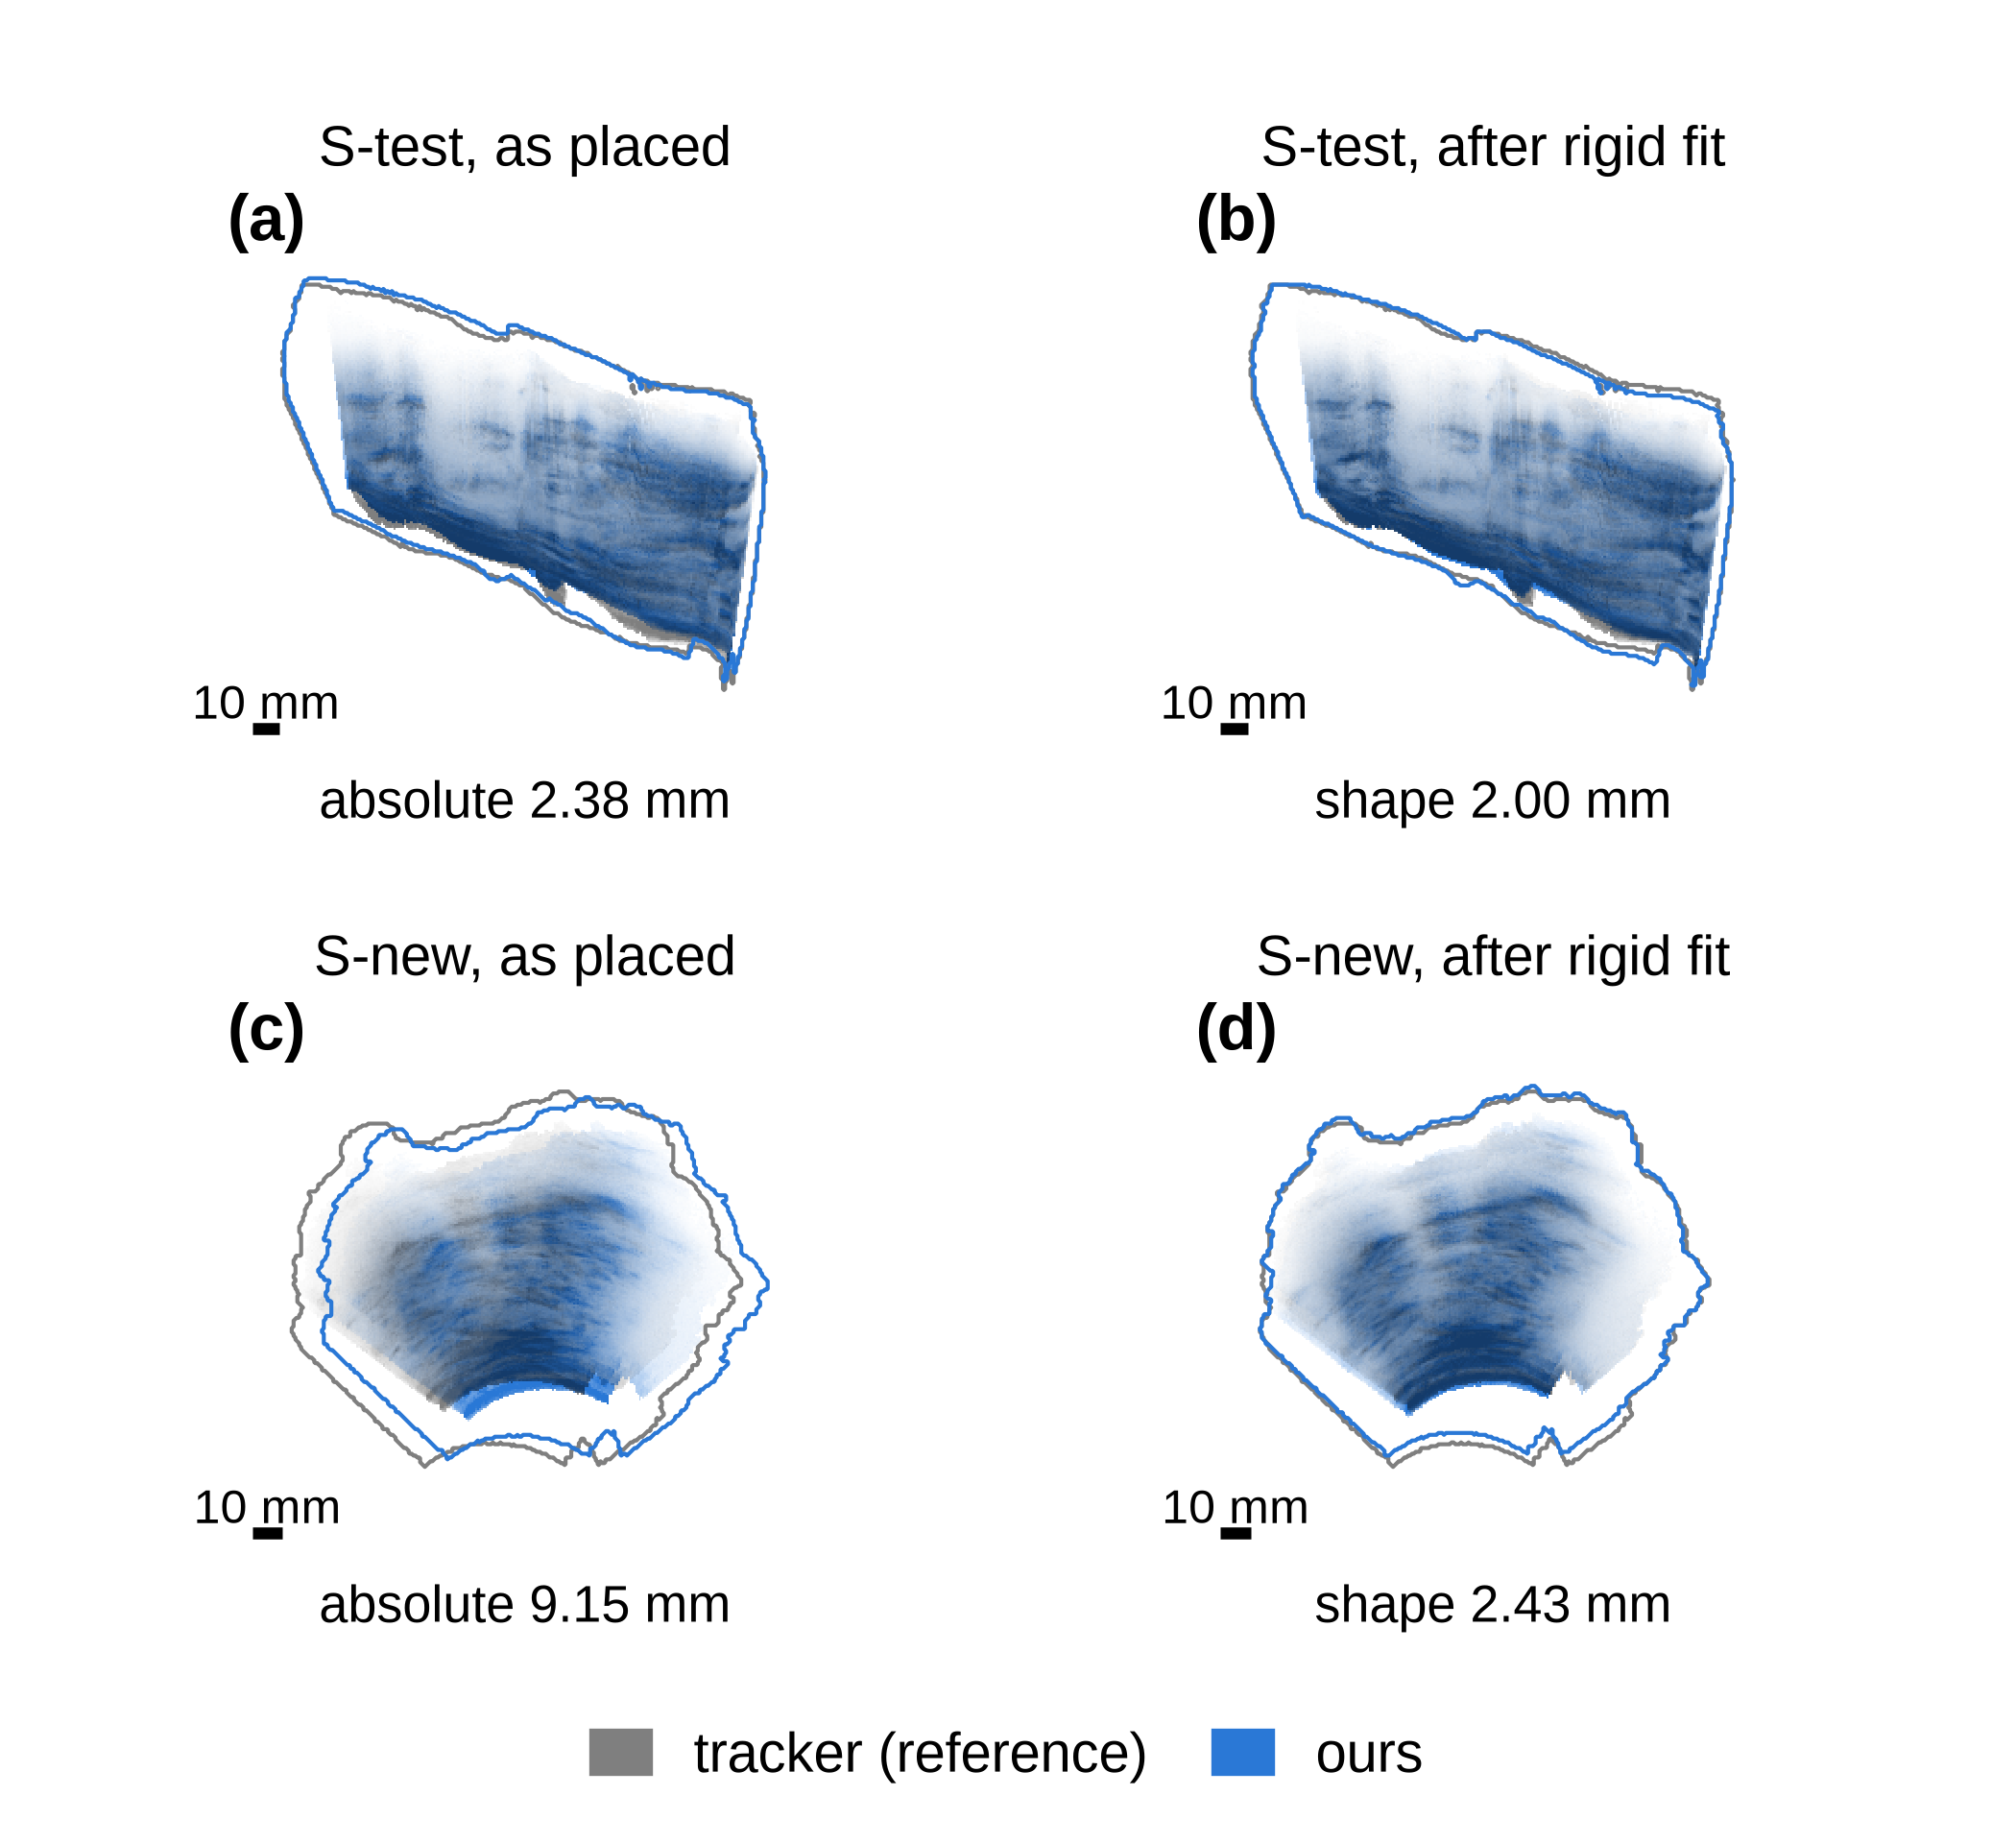
\includegraphics[width=0.90 \linewidth]{fig_volume_snew.png}
  \caption{Volumes as placed (left) and after the best rigid fit of the sweep (right); tracker poses grey, proposed system blue. (a,~b)~\Ftest{} sweep: 2.38 / 2.00\,mm. (c,~d)~\Ftwo{} sweep, short generic scan: 9.15 / 2.43\,mm. The rows use different viewing directions.}
  \label{fig:volume_snew}
\end{figure}

\subsection{Ablation Study}
\label{sec:res_ablation}\label{sec:res_mapping}\label{sec:res_tracking}\label{sec:res_calib}
The lower part of Table~\ref{tab:test} summarises the ablations.

\subsubsection{Self-Mapping} Self-mapping placed all 3356 \Ftest{} room-scan frames, 92\,\% after the first round and 100\,\% after the second. In the test sessions, it stopped after one to three rounds. Compared with the tracker, the map error was 2.0\,mm at the camera centre, 2.6\,mm at points 1\,m in front of the camera and $0.19^\circ$ in orientation, and the error of the relative motion over 1\,s was 1.5\,mm. Mapped again from scratch without loop closures, the \Ftest{} tracking error increased from 2.34 / 1.72 to 5.77 / 3.18\,mm; without the camera correction $\Tcorr$, it increased to 11.49 / 4.08\,mm. Thus, loop closures and the camera correction each carry a large part of the accuracy.

\subsubsection{Tracking} With the oracle map on \Fval{}, training for 30, 60 and 120 epochs gave an anchor error of 6.3, 5.4 and 5.1\,mm, and Kabsch with depth instead of PnP reduced it further to 3.4\,mm. A first training recipe, with a half-precision head and 15 epochs, gave 15.8\,mm. Geometric augmentation increased the anchor error from 3.4 to 6.5\,mm, and full-resolution input ($720\times1280$, 30 epochs) from 6.3 to 7.3\,mm. On \Ftest{}, smoothing reduced the jitter from 1.67 to 0.93\,mm and the tracking error from 2.03 to 1.85\,mm. Learned odometry was 0.3--0.6\,mm less accurate than classical odometry. Thus, the settings of Table~\ref{tab:params} are those with the lowest anchor error on \Fval{}.

\subsubsection{Camera Correction} When fitted on each \Ftest{} scan alone, $\Tcorr$ agreed within 1.8\,mm and $0.05^\circ$, and each fit remained valid on the other scan, with a scene-point error of 2.9\,mm. When fitted on \Ftwo{}, its rotation differed by about $0.5^\circ$. Refitting $\Tcorr$ on \Flarge{} reduced the error from 9.40 to 7.87\,mm on \Flarge{} and from 11.54 to 9.58\,mm on \Fsubj{}. Thus, one $\Tcorr$ carries over between sessions, and part of the placement error remains.

\begin{table*}[!tb]
  \caption{Coverage, scene changes and occlusion: tracking error (mm, lower is better), absolute / shape. Cov.: coverage of the sweep viewpoints; map err.: camera error of the self-made map (mm). Bold: exam-view scan, the protocol. Occluder rows: mean (worst sweep) / shape.}
  \label{tab:ctrl}\label{tab:coverage}\label{tab:changes}\label{tab:occlusion}
  \centering
  \begin{tabular}{@{}llcccc@{}}
    \toprule
    Sweeps & Map & Cov. & Map err. & Proposed & Oracle\\
    \midrule
    \multicolumn{6}{@{}l}{\emph{Coverage: exam-view, generic and both scans (phantom); short generic scans (\Ftwo{})}}\\
    \Pref{} & \textbf{exam-view scan} & 96\,\% & 2.7 & \textbf{2.28 / 1.90} & 1.85 / 1.67\\
     & generic scan & 0\,\% & 6.5 & 13.57 / 3.79 & 10.95 / 3.93\\
     & both scans in one map & 96\,\% & 3.4 & 3.15 / 1.81 & --\\
    \Prearra{} & \textbf{exam-view scan} & 75\,\% & 2.4 & \textbf{4.43 / 2.81} & --\\
     & generic scan & 93\,\% & 2.2 & 3.36 / 2.46 & --\\
    \Prearrb{} & \textbf{exam-view scan} & 96\,\% & 2.2 & \textbf{3.11 / 1.76} & --\\
     & generic scan & 78\,\% & 5.2 & 6.35 / 1.76 & --\\
    \Ppeople{} & \textbf{exam-view scan} & 98\,\% & 2.2 & \textbf{2.24 / 1.70} & --\\
     & generic scan & 100\,\% & 5.2 & 5.07 / 1.28 & --\\
    \Pempty{} & \textbf{exam-view scan} & 92\,\% & 4.3 & \textbf{5.85 / 3.04} & --\\
     & generic scan & 97\,\% & 10.9 & 13.03 / 2.83 & --\\
    \Fnew{} (8) & own generic scans & $\le$14\,\% & -- & 5.04 / 2.94 & 5.14 / 2.92\\
    \Fsmall{} (4) & own generic scans & $\le$14\,\% & -- & 6.55 / 2.40 & 5.77 / 2.66\\
    \Flarge{} (4) & own generic scans & $\le$14\,\% & -- & 9.40 / 2.05 & 5.63 / 2.96\\
    \Fsubj{} (6) & \Flarge{}'s scans & $\le$14\,\% & -- & 11.54 / 3.10 & 9.63 / 3.16\\
    \Farm{} (4) & \Flarge{}'s scans & $\le$14\,\% & -- & 7.07 / 2.98 & 6.25 / 4.16\\
    \Ftwo{} mean (26) & & 0--14\,\% & -- & 7.92 / 2.69 & 6.48 / 3.17\\
    \midrule
    \multicolumn{6}{@{}l}{\emph{Scene changes: scan after the sweeps, outdated map (phantom)}}\\
    \Pref{} & own, scanned after the sweeps & -- & 2.0 & 2.50 / 1.96 & --\\
    \Prearra{} & \Pref{}'s map & 91\,\% & -- & 4.28 / 3.00 & --\\
    \Prearrb{} & \Pref{}'s map & 84\,\% & -- & 59.4 (21\,\% posed) & --\\
    \Prearrb{} & \Prearra{}'s map & 94\,\% & -- & 40.9 (96\,\% posed) & --\\
    \Pempty{} & \Prearrb{}'s map & 96\,\% & -- & 13.9 (p90 46.6) & --\\
    \midrule
    \multicolumn{6}{@{}l}{\emph{Occlusion: synthetic occluder, share of the image width (phantom, exam-view scan)}}\\
    \Prearra{} & none & -- & -- & 4.43 (6.3) / 2.81 & --\\
     & 30\,\% & -- & -- & 5.16 (7.5) / 3.38 & --\\
     & 60\,\% & -- & -- & 5.28 (8.5) / 3.88 & --\\
    \Prearrb{} & none & -- & -- & 3.11 (5.1) / 1.76 & --\\
     & 30\,\% & -- & -- & 3.54 (6.1) / 2.27 & --\\
     & 60\,\% & -- & -- & 3.89 (6.6) / 2.80 & --\\
    \bottomrule
  \end{tabular}
\end{table*}

\subsection{Coverage of the Examination Views}
\label{sec:res_coverage}
\subsubsection{Controlled Coverage} Fig.~\ref{fig:coverage_error} shows the error of every phantom map against the coverage of the sweep viewpoints, and the upper part of Table~\ref{tab:ctrl} gives the values. On the same 8 \Pref{} sweeps, the exam-view scan covered 96\,\% of the sweep viewpoints and gave 2.28 / 1.90\,mm with the self-made map and 1.85 / 1.67\,mm with the oracle map. The generic scan covered 0\,\% and gave 13.57 / 3.79\,mm with the self-made map and 10.95 / 3.93\,mm with the oracle map (the exam-view map was lower on all 8 sweeps; Wilcoxon $p=0.0078$). As shown in Fig.~\ref{fig:volume}, the volume from the generic map was displaced but kept its shape, and every frame passed the inlier gate. With both scans in one map, the error was 3.15 / 1.81\,mm, and the camera error of the map increased from 2.7 to 3.4\,mm.

Over all current phantom maps, the shape error ranged from 1.28 to 3.79\,mm. With at least 90\,\% coverage, the absolute error was about the camera error of the map plus 1\,mm (Fig.~\ref{fig:coverage_error}b). The exam-view scan gave the lower error in every set except \Prearra{}, where it covered 75\,\% and the generic scan 93\,\% (4.43 vs.\ 3.36\,mm). The emptied room \Pempty{} gave the largest map errors, 4.3\,mm with the exam-view scan and 10.9\,mm with the generic scan. At the frame level, with the oracle map of an earlier network version, the median anchor error within the same session was 2.3--5.6\,mm for sweep frames within 30\,mm and $10^\circ$ of a room-scan pose, and 5.7--9.1\,mm for the other frames (\Fval{}, \Ftest{}, \Fnew{} and \Fsmall{}). Using only the first 20, 40 and 60\,s of each \Ftest{} scan gave 3.00, 2.03 and 1.85\,mm, respectively (further views in the supplementary material). Thus, coverage rather than mapping sets the error: with perfect labels, the generic scan still gave 10.95\,mm.

\begin{figure}[t]
  \centering
  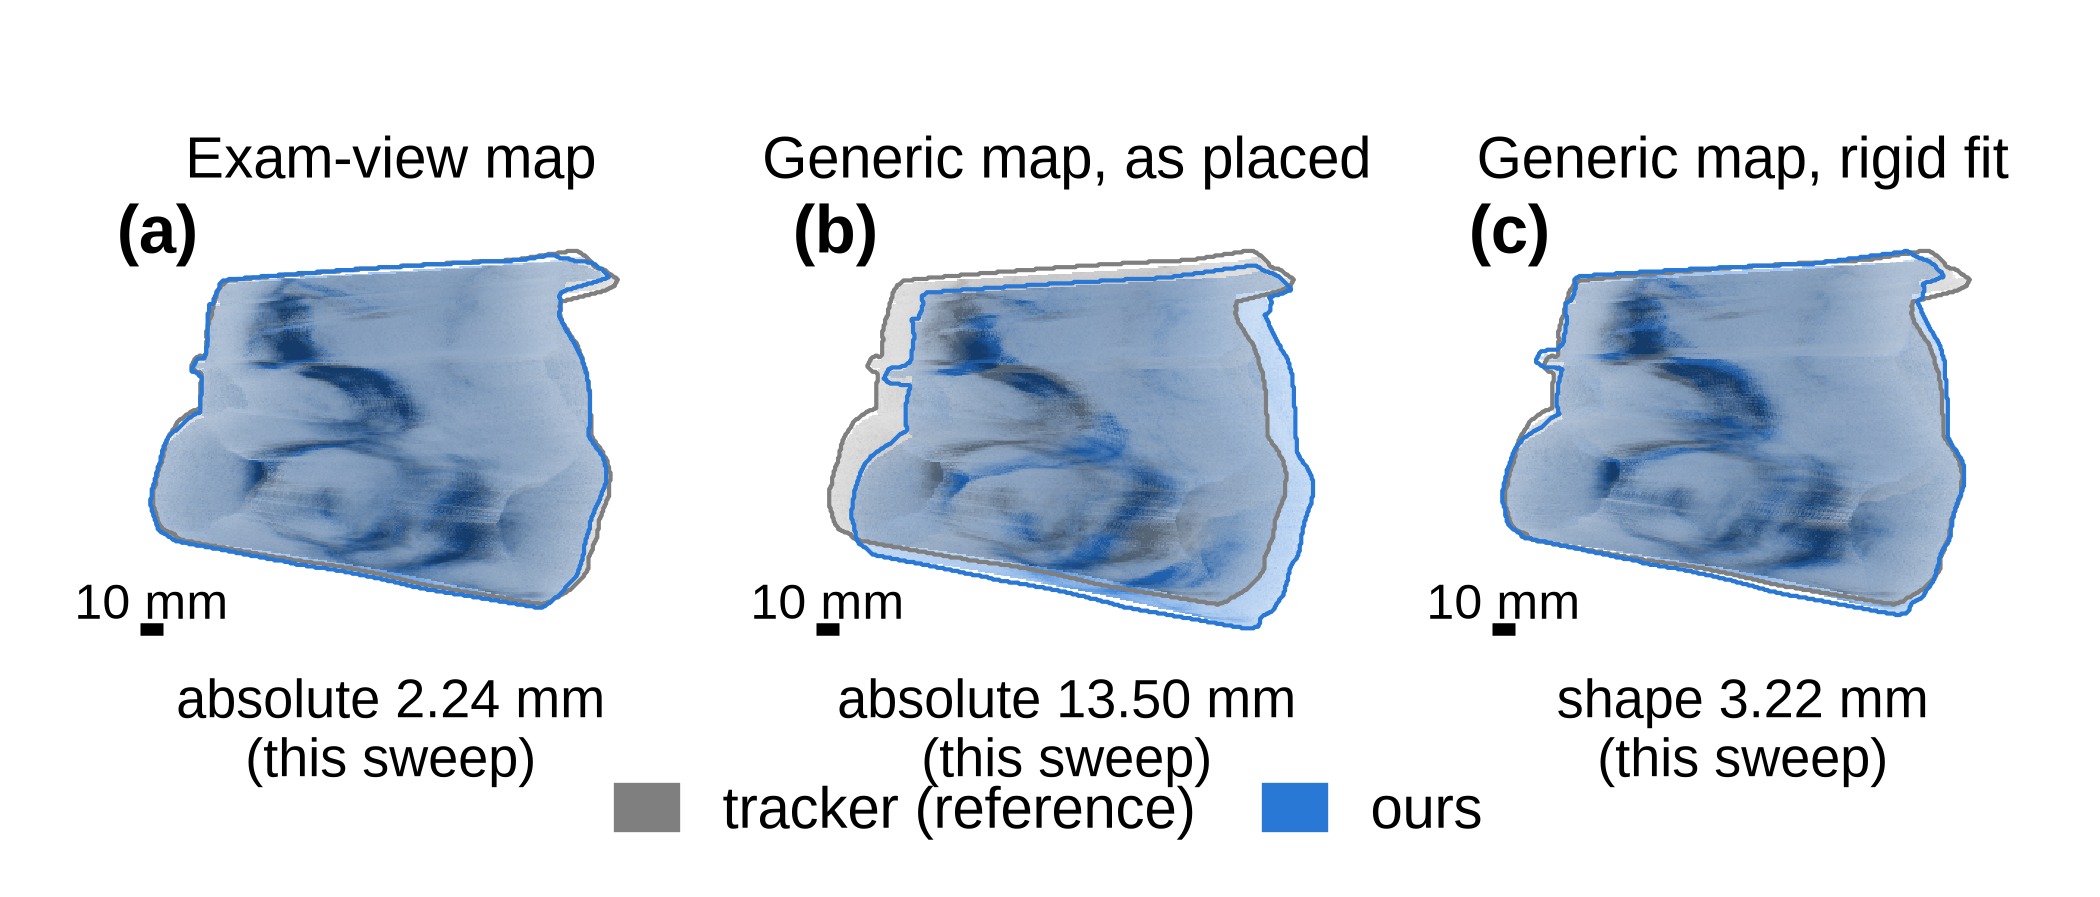
\includegraphics[width=0.96 \linewidth]{fig_volume_coverage.png}
  \caption{One \Pref{} sweep, tracker poses (grey) and proposed system (blue), seen from the skin. (a)~Exam-view map. (b)~Generic map. (c)~Generic map after the best rigid fit of the sweep.}
  \label{fig:volume}
\end{figure}

\begin{figure}[t]
  \centering
  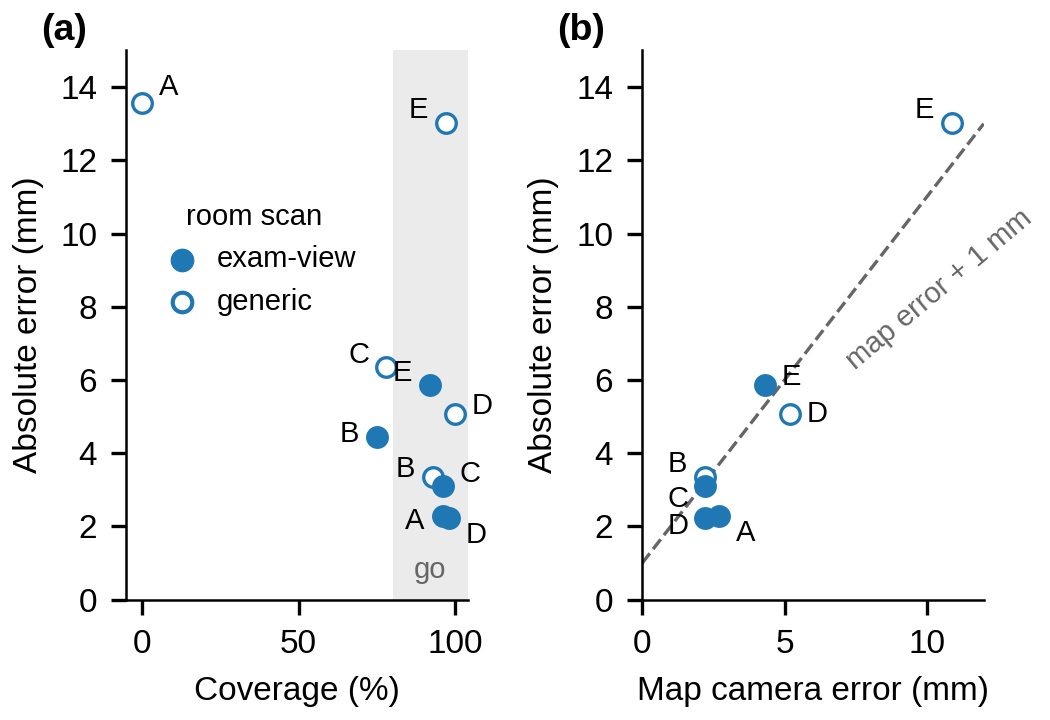
\includegraphics[width=0.90 \linewidth]{fig_coverage_error.png}
  \caption{Phantom maps (filled: exam-view scan; open: generic scan). (a)~Error against coverage; shaded: go region of the coverage check. (b)~Maps with $\ge90$\,\% coverage: error against the camera error of the map; dashed: map error + 1\,mm.}
  \label{fig:coverage_error}
\end{figure}

\subsubsection{Short Generic Scans} On \Ftwo{}, whose short generic scans covered 0--14\,\% of the sweep viewpoints, self-mapping placed every room-scan frame. The mean error was 7.92 / 2.69\,mm (absolute $7.92\pm2.56$\,mm over the five sets) for the proposed system, 6.48 / 3.17\,mm for the oracle map and 4.76 / 3.34\,mm for the classical pipeline. Among these three, the proposed system had the lowest shape error, also on every set except \Fnew{} (2.94 vs.\ 2.92\,mm), and the highest absolute error. The largest error occurred on the second volunteer, \Fsubj{} (11.54 / 3.10\,mm). Fig.~\ref{fig:volume_snew}c,d shows an \Ftwo{} sweep. Thus, without covering scans, the error is more a placement of the whole sweep than a distortion of it.

\subsection{Scene Changes}
\label{sec:res_changes}
People moving in the background (\Ppeople{}, 2.24\,mm) and recording the room scan after instead of before the sweeps (\Pref{}, 2.50\,mm, map error 2.0\,mm) did not increase the error. The maps of earlier sets covered 84--96\,\% of the views of later sets (Table~\ref{tab:ctrl}, middle part). \Pref{}'s map on \Prearra{} gave 4.28 / 3.00\,mm, similar to \Prearra{}'s own scans. \Pref{}'s map on \Prearrb{} gave 59.4\,mm with 21\,\% of the frames posed, and \Prearra{}'s map on \Prearrb{} gave 40.9\,mm with 96\,\% posed. \Prearrb{}'s map on \Pempty{} gave 13.9\,mm, with a 90th percentile of 46.6\,mm. Rescanning restored the error on \Prearrb{} to 3.11\,mm. The 400-inlier gate did not catch these failures, but the median inlier count separated them: it ranged from 1371 to 2213 for current maps, was 1126 for \Pref{}'s map on \Prearra{}, and ranged from 23 to 450 for the failing cases (Fig.~\ref{fig:volume_outdated}). Thus, a very large change makes a map outdated, and the median inlier count detects it where the inlier gate does not.

\begin{figure}[t]
  \centering
  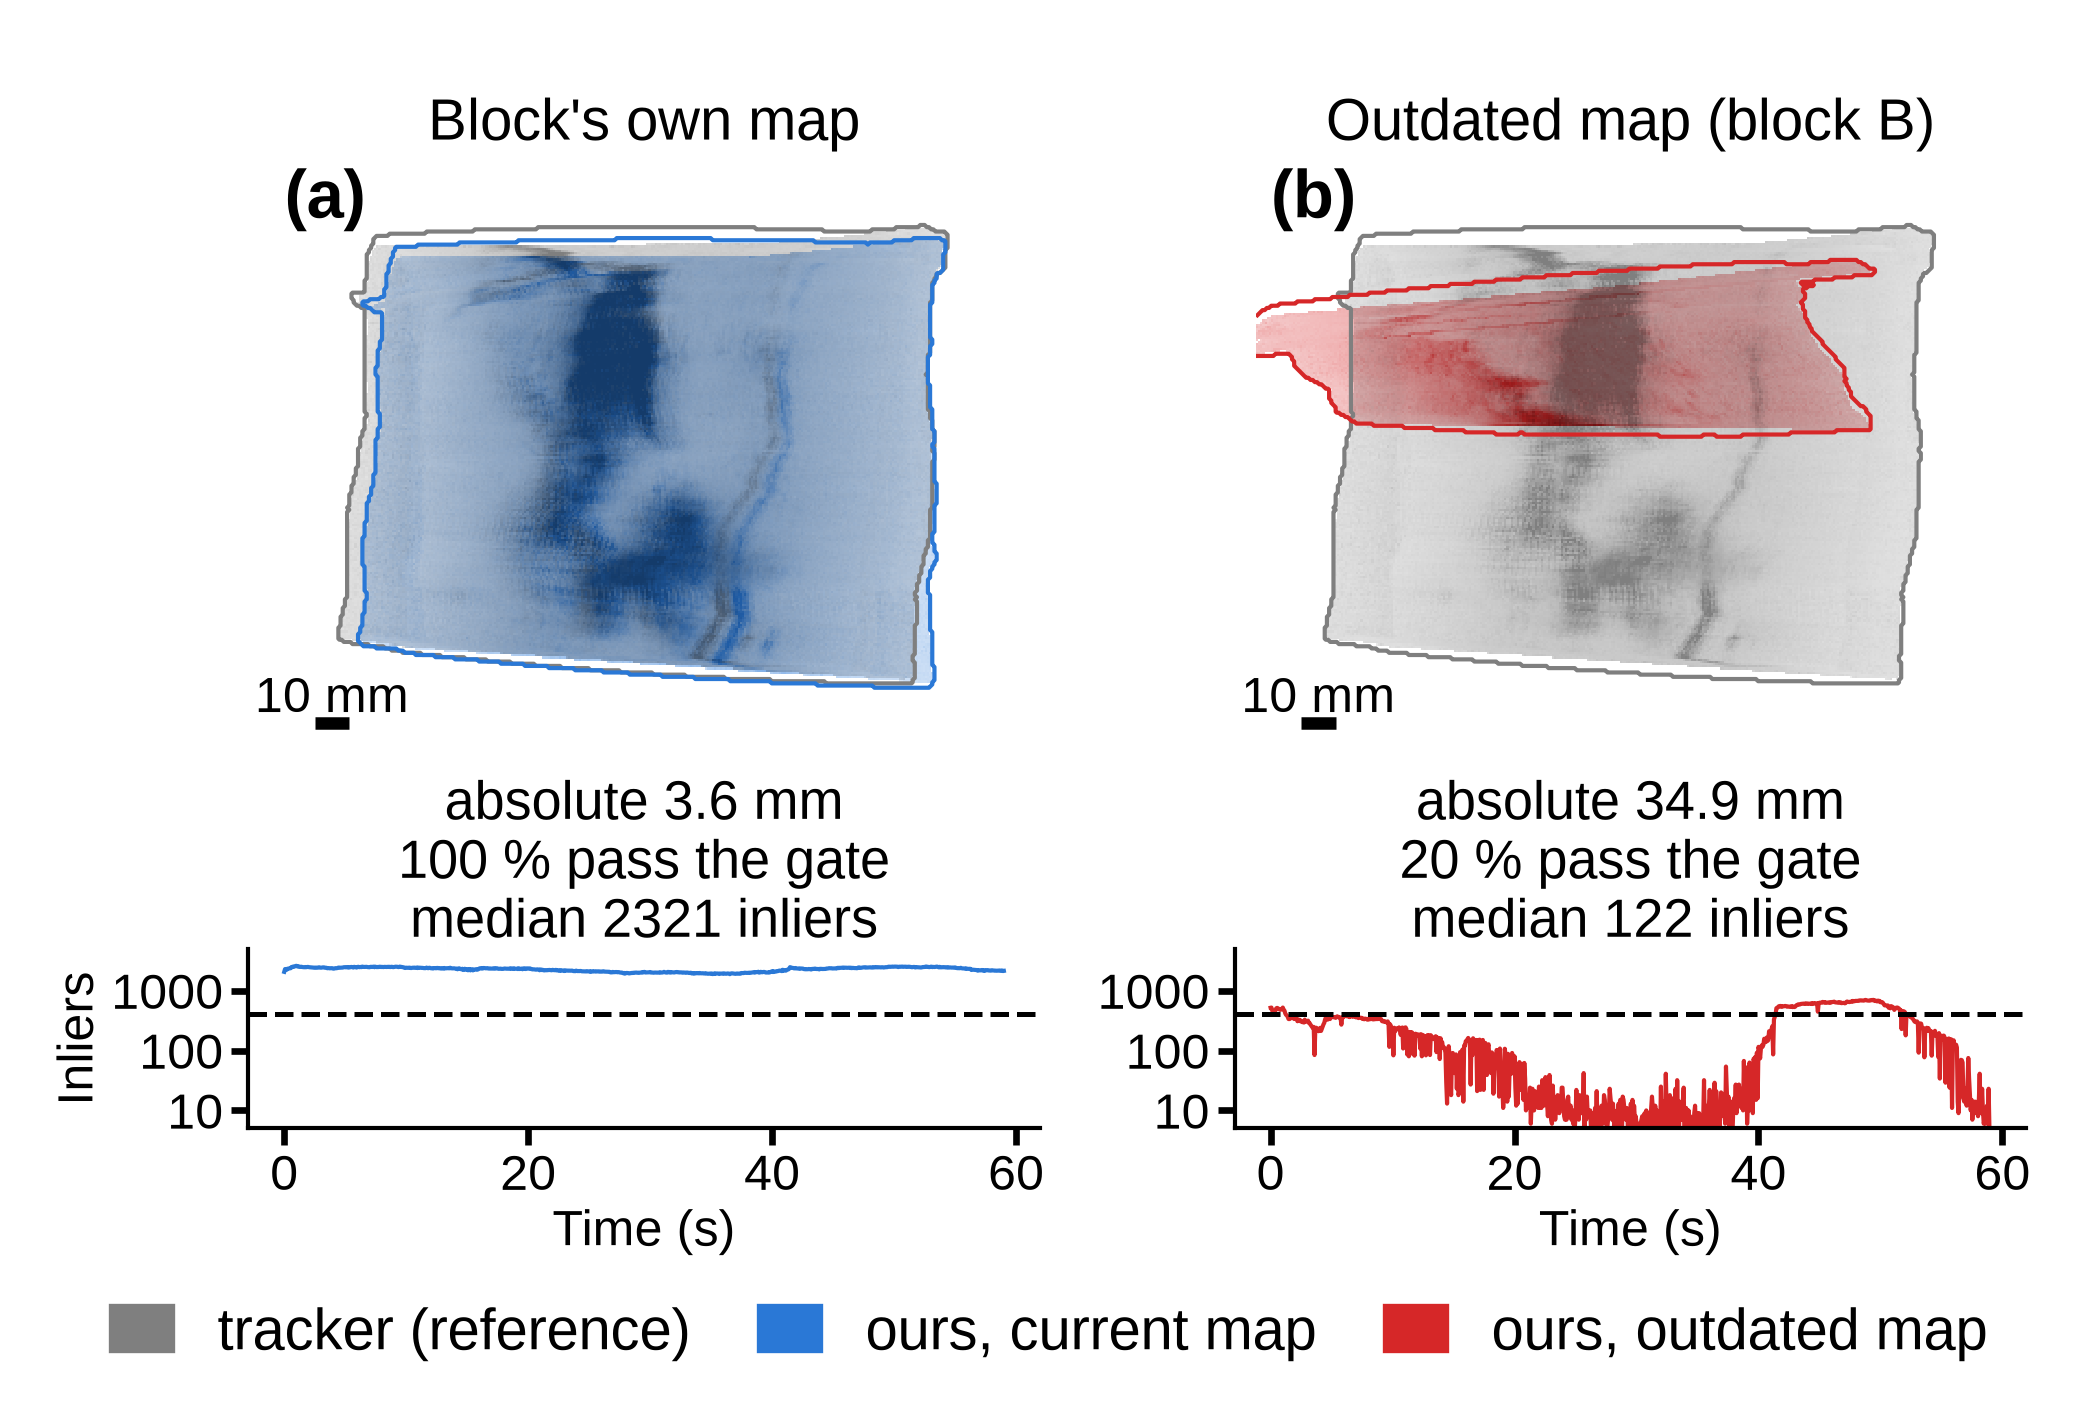
\includegraphics[width=0.90 \linewidth]{fig_volume_outdated.png}
  \caption{A \Prearrb{} sweep with its own map (a, 3.6\,mm, all frames pass the gate) and with \Prearra{}'s outdated map (b, 34.9\,mm, 20\,\% pass); below, Kabsch inliers per frame, 400-inlier gate dashed. Median inliers: 2321 and 122.}
  \label{fig:volume_outdated}
\end{figure}

\subsection{Occlusion}
\label{sec:res_occlusion}
With the synthetic occluder (Table~\ref{tab:ctrl}, lower part), the mean error of the proposed system increased by 0.4--0.9\,mm, no sweep exceeded 8.5\,mm, and 87--100\,\% of the frames were posed. ORB-SLAM3 in localisation only, given the same frames, had the lower mean error in three of the four occluded settings, but it failed on single sweeps while reporting every frame as tracked: on \Prearra{}, its worst sweep was 132.2\,mm off with 30\,\% of the image width occluded and 12.9\,mm off with 60\,\%. With 60\,\% occluded on \Prearra{}, the shape error was 3.88\,mm for the proposed system and 8.44\,mm for ORB-SLAM3. The other ORB-SLAM3 modes also failed on single sweeps, with worst sweeps of 38.6 and 39.7\,mm (supplementary material).

On \Farm{}, a real arm crossed the view in two sweeps. On one of these sweeps, ORB-SLAM3 was 81.5\,mm off in one run and 28.2\,mm in another, while the proposed system was 6.9\,mm off. Thus, under occlusion the proposed system stayed within a bounded error, whereas ORB-SLAM3, with the lower mean error, lost single sweeps while reporting tracking.

\begin{table}[!tb]
  \caption{Comparison with other trackers: absolute tracking error (mm, lower is better), \Ftest{} shape error (mm) and jitter (\Ftest{} / \Ftwo{}, mm). Upper part: maps labelled with tracker poses; lower part: no tracker-made map. Bold: best per column in each part.}
  \label{tab:baselines}
  \centering
  \scriptsize
  \setlength{\tabcolsep}{1.8pt}
  \begin{tabular}{@{}lcccccc@{}}
    \toprule
    System & \Fval & \Ftest & Shape & Strict & \Ftwo & Jitter\\
    \midrule
    \multicolumn{7}{@{}l}{\emph{Tracker-made map}}\\
    Odometry only & 37.0 & 9.4 & 6.23 & 9.8 & 12.2 & --\\
    Pose regression & -- & 8.5 & -- & -- & 44.2 & --\\
    Classical anchors + odometry & 4.2 & 3.1 & 2.47 & 3.0 & \textbf{4.76} & 1.09 / 1.28\\
    Hybrid: SCR anchors + odometry & 4.2 & 2.6 & -- & -- & 6.54 & 1.08 / 1.29\\
    SCR on every frame (oracle map) & \textbf{3.35} & \textbf{1.85} & \textbf{1.57} & \textbf{2.98} & 6.48 & \textbf{0.93} / \textbf{1.15}\\
    \midrule
    \multicolumn{7}{@{}l}{\emph{No tracker-made map}}\\
    Proposed, self-mapped & -- & 2.34 & 1.72 & \textbf{2.94} & 7.92 & 0.90 / --\\
    Classical, self-made map & -- & 3.65$^{a}$ & 2.66$^{a}$ & -- & \textbf{5.78} & --\\
    ORB-SLAM3, localisation only & -- & \textbf{1.84} & \textbf{1.30} & -- & 8.37 & \textbf{0.68} / --\\
    \bottomrule
  \end{tabular}\\[2pt]
  \raggedright\footnotesize $^{a}$Proposed system 2.35 / 1.73\,mm on the same frames.
\end{table}

\subsection{Comparison With Other Trackers}
\label{sec:res_compare}\label{sec:res_slam}
Table~\ref{tab:baselines} summarises the comparison. In its upper part, every system uses a map labelled with tracker poses, so that only the localisation method differs; its lower part contains the systems that need no tracker. Per-set \Ftwo{} errors of all systems are given in the supplementary material. On \Ftest{}, the classical pipeline reached 3.11 / 2.47\,mm and odometry only, the lower bound, 9.43 / 6.23\,mm. Between nearby frames, all systems agreed: the out-of-plane error over 8 / 30 rows was 0.29 / 0.62\,mm for the classical pipeline and 0.28 / 0.54\,mm for odometry only, against 0.37 / 0.62\,mm for the proposed system.

\subsubsection{Learned and Classical Localisers} As single-image localisers, the SCR anchors were about $8\times$ more accurate than the pose-regression anchors, with 1.8 vs.\ 15.3\,mm on \Ftest{} and 6.0 vs.\ 49.0\,mm on \Ftwo{}. The SCR anchors gave a pose for every frame, whereas the pose-regression anchors were accepted for 37--93\,\% of the frames. Classical anchors reached 2.6\,mm on \Ftest{} and 5.3\,mm on \Ftwo{}. One SCR network on every frame was more accurate than the hybrid of SCR anchors and odometry on \Fval{} (3.35 vs.\ 4.2\,mm) and \Ftest{} (1.85 vs.\ 2.6\,mm), and similar on \Ftwo{} (6.48 vs.\ 6.54\,mm), with lower jitter.

Compared with the classical pipeline, SCR was more accurate on \Fval{} (3.35 vs.\ 4.2\,mm) and \Ftest{} (1.85 vs.\ 3.1\,mm), equally accurate under the strict protocol (2.98 vs.\ 3.0\,mm), and less accurate on \Ftwo{} (6.48 vs.\ 4.76\,mm). The shape error of SCR was lower on every set. Without a tracker, the classical pipeline on the self-made map gave 3.65 / 2.66\,mm on \Ftest{}, compared with 2.35 / 1.73\,mm for the proposed system on the same frames, and 5.78\,mm on \Ftwo{}, compared with 7.92\,mm for the proposed system. Results with pooled room scans are given in the supplementary material. Thus, SCR was the more accurate with covered views, and the classical pipeline with uncovered views.

\subsubsection{US-Only Motion Estimation} The US-only method of Li et al.\ \cite{li2024longterm} reproduced its published accuracy on its own data (21.4 vs.\ 22.8\,mm). On the sweeps of this study, it was no more accurate than assuming no motion: it gave 129\,mm zero-shot, 75--125\,mm fine-tuned and 49--56\,mm trained from scratch, compared with 49--58\,mm for zero motion. Networks with US input, alone or fused with RGB, did not improve on RGB alone, and the best fusion weight of the US estimate was zero. Between nearby frames, the camera was more accurate than speckle decorrelation (0.07 / 0.19 / 0.24\,mm vs.\ 0.19 / 0.78 / 1.83\,mm over 1 / 4 / 8 frames).

\subsubsection{SLAM Reference} ORB-SLAM3 in localisation only reached 1.84, 8.37 and 2.36\,mm on \Ftest{}, \Ftwo{} and the phantom, compared with 2.34, 7.92 and 3.58\,mm for the proposed system; on \Ftwo{} without \Farm{}, it reached 4.45\,mm. With each frame relocalised, it was lower on 52 of 63 sweeps, on average by 1.96\,mm (95\,\% bootstrap interval 1.30--2.61\,mm; Wilcoxon $p<0.001$). With the generic \Pref{} scan, it gave 2.88\,mm, compared with 13.57\,mm. Relocalising one frame took it 25--41\,ms on the CPU (median). Thus, its advantage lies in the map rather than in tracking over time.


%======================================================================
\section{Discussion}
\label{sec:discussion}
%======================================================================
% This study investigates whether a probe-mounted RGB-D camera can replace the external tracker in freehand 3D US. With a room scan covering the examination views in a furnished room, the proposed system reached a tracking error of 2.2--3.1\,mm and a shape error of 1.7--1.9\,mm, with nothing outside the probe during the examination. Removing the tracker from mapping cost 0.4--0.5\,mm relative to the same network trained on tracker poses, so self-mapping is not the main limit. The results also show when the approach should not be used, and how this can be detected before or during the examination.

\subsection{Design Choices}
\label{sec:design}
Loop closures and the camera correction $\Tcorr$ were both essential: without them the error rose to 5.77 and 11.49\,mm. End-to-end training through the Kabsch fit, as in DSAC* \cite{brachmann2022dsac}, was not needed, because the map rather than the solver limits the accuracy. No temporal model is learned: odometry added nothing once every frame has an absolute pose, and a fixed robust smoother reduces the jitter. Poses are refined by the pose graph only, not jointly with the network as in ACE0 \cite{brachmann2024ace0}, because joint refinement made an \Ftest{} map less accurate (camera position 8.4 to 8.9\,mm). $\Tcorr$ is needed once per probe; its transfer across sessions adds part of the placement error (\Flarge{}, 9.40 vs.\ 7.87\,mm after refitting).

\subsection{Coverage Sets the Accuracy}
A network that learns the room from a scan is accurate only near the viewpoints of that scan. With perfect labels, a scan that missed the examination views still gave 10.95\,mm instead of 1.85\,mm, and at the frame level the anchor error was higher away from the room-scan poses (5.7--9.1 vs.\ 2.3--5.6\,mm). This is a limit of regressing scene coordinates, not of self-mapping, and it is consistent with the larger errors on \Ftwo{}, whose short generic scans covered at most 14\,\% of the views. For the operator, the consequence is concrete: the room scan should follow the planned sweep paths, which takes 1--2\,min. More footage did not substitute for the right footage: adding a generic scan made the map worse (3.15 vs.\ 2.28\,mm). Once coverage is sufficient, the error follows the camera error of the map plus about 1\,mm, so an emptied room, where depth ICP has little structure to align, gave a poorer map (5.85\,mm). Training that lets scene coordinate networks extrapolate to new viewpoints, as ACE-G does for RGB \cite{bruns2025aceg}, is the most direct way to relax the coverage requirement.

Without coverage, the error is mostly a placement of the whole sweep rather than a distortion of it: on \Ftwo{}, the proposed system had the lowest shape error of the three map-based systems but the largest absolute error, and between nearby frames all systems agreed (0.28--0.37\,mm). For volume measurements that need no registration to other images, shape is the relevant error; for navigation in a room frame, the absolute error is.

\subsection{Bounded and Detectable Failures}
Because every frame is localised on its own, a wrong pose is not carried into the next frame. Under occlusion, the mean error of the proposed system rose by at most 0.9\,mm and no sweep exceeded 8.5\,mm; with a real arm in view on \Farm{}, the error stayed at 6.9\,mm on the sweep where ORB-SLAM3 failed. People moving in the background, a scan recorded after the sweeps and an earlier map after a large change (\Pref{}'s map on \Prearra{}) did not increase the error notably. The failures that remain have causes that can be checked. An outdated map after a very large change gave low inlier counts (median 23--450, against 1371--2213 for current maps), which the map-age check flags without a tracker. Low coverage, in contrast, is silent: every frame passed the inlier gate, so the coverage check is needed.

\subsection{Comparison With Other Trackers}
Among the learned options, SCR was clearly the most accurate: its anchors were about $8\times$ more accurate than those of pose regression. A pose-regression network merges the whole image into one pose, which moved objects or hands corrupt, whereas SCR predicts 3600 independent correspondences, RANSAC keeps the consistent ones, and a rigid fit through thousands of them averages the noise. The US images added no information to the camera pose in this set-up: between nearby frames the camera was already more accurate than speckle decorrelation, and over a sweep a US-only estimate was no better than assuming no motion. The classical pipeline and SCR fail in different ways. SIFT copes better with views the room scan does not cover (\Ftwo{}, 4.76 vs.\ 6.48\,mm with tracker-made maps), but it confidently matches objects that have since moved, so with pooled room scans it broke, whereas the SCR network improved (supplementary material). With covered views and a self-made map, SCR was more accurate (2.35 vs.\ 3.65\,mm on \Ftest{}).

ORB-SLAM3, as an established SLAM reference, was more accurate on most sweeps, also when both systems used only the room scan. The difference lies in the map rather than in tracking over time, since ORB-SLAM3 kept its accuracy with every frame relocalised: sparse keypoints with descriptors generalise to viewpoints the room scan missed (2.88 vs.\ 13.57\,mm with the generic scan), and a network that regresses room coordinates does not. What the per-frame approach offers instead is a different failure behaviour. ORB-SLAM3 occasionally lost a whole sweep by 13--132\,mm while reporting successful tracking, and such failures varied from run to run (81.5 and 28.2\,mm on the same sweep). For compounding, a silent failure of a whole sweep is harder to handle than a known, bounded error. The two approaches are therefore complementary: an independent per-frame check could guard a SLAM system, and scene coordinate relocalisation can be used inside SLAM, as in ACE-SLAM \cite{alzugaray2025aceslam}.

\subsection{Limitations and Future Work}
Several limitations remain. First, preparation per room takes about 30\,min of self-mapping and 13--40\,min of training, and tracking runs at 60--70\,ms per frame; real time was shown on recorded data, not live, so a live implementation is the next step. Second, all data come from one room, two subjects and one phantom, and the test sets are small (32 phantom and 31 forearm sweeps); more rooms and subjects are needed. Third, the occlusion experiment uses one synthetic occluder on two phantom sets, and real hands and arms differ in shape, motion and depth; the real case, \Farm{}, has two sweeps with an arm in view. Finally, $\Tcorr$ and the coverage check used the tracker; a tracker-free coverage check is future work.

The network already takes RGB only; depth enters the labels, the Kabsch fit, ICP and the pose graph. A probe camera without depth would be smaller and cheaper and would avoid depth failures on shiny surfaces. Its cost at test time is that PnP replaces the Kabsch fit, which on \Fval{} raised the anchor error from 3.4 to 5.1\,mm with the oracle map; mapping without depth, as in ACE0 \cite{brachmann2024ace0}, is the remaining step. Validation in more rooms, on more subjects and in live use is the next step towards clinical use.


%======================================================================
\section{Conclusion}
\label{sec:conclusion}
%======================================================================
This paper presented a tracker-free approach for freehand 3D US, in which a probe-mounted RGB-D camera and one scene coordinate network that maps its own room scan give the pose of every US frame. Experiments were conducted on a phantom and on the forearms of two volunteers, against an optical tracker. The results show that coverage decides the accuracy, then map quality, then scene changes; an exam-view scan, a coverage check and an inlier check make these conditions explicit before the examination. Future work will focus on scene coordinate networks that generalise to new viewpoints, an RGB-only probe camera and the combination with SLAM, followed by validation in more rooms and on more subjects.


% \section*{Acknowledgment}    



\bibliographystyle{IEEEtran}
\bibliography{bib}


\end{document}